

\section*{Appendix A: proofs}

\subsection*{Proof of Theorem \ref{TeoremaMartingale}}
For all $ u \in \mathcal{I}_{T}$ we have
\begin{equation}
\mathbb{E}\left[ M^{u}_{T}\right]=\mathbb{E}\left[e^{-\tr\left[ u\Sigma_{T}\right]} \right]<\infty,\nonumber
\end{equation}
and by the affine property we obtain
\begin{align}
\mathbb{E}\left[ M^{u}_{T}|\mathcal{F}_{t}\right]&=\mathbb{E}\left[ \exp\left\{-\phi_{T-T}(u)-\tr\left[\psi_{T-T}(u)\Sigma_{T} \right]\right\}|\mathcal{F}_{t}\right]\nonumber\\
&=\mathbb{E}\left[\exp\left\{-\tr\left[u\Sigma_{T} \right] \right\} |\mathcal{F}_{t}\right]\nonumber\\
&=\exp\left\{ -\phi_{T-t}(u)-\tr\left[ \psi_{T-t}(u)\Sigma_{t}\right]\right\}=M^{u}_{t},\nonumber
\end{align}
hence the process is a martingale. Now we show that $M_{t}^{u}>1$. Recall that by assumption $u\in \mathcal{I}_{T}\cap S_{d}^{--}$ and 
\begin{equation}
M^{u}_{t}=\mathbb{E}\left[\exp\left\{-\tr\left[u\Sigma_{T} \right] \right\} |\mathcal{F}_{t}\right],\nonumber\\
\end{equation}
so that if $-\tr\left[u\Sigma_{T} \right]>0$ a.s. then we are done.
We proceed as in \cite{article_gou02} and apply the singular value decomposition to the negative definite matrix $u$, i.e. $u$ may be written as:
\begin{equation}
u=\sum_{i=1}^{n}{\lambda_{i}u_{i}u_{i}^{\top}}\nonumber
\end{equation}
where $\lambda_{i}$ are the eigenvalues of $u$ and $u_i$ are the eigenvectors. By assumption $\Sigma_{T}$ takes values in $S_{d}^{++}$, hence
\begin{align}
-\tr\left[u\Sigma_{T} \right]&= -\tr\left[ \sum_{i=1}^{n}{\lambda_{i}u_{i}u_{i}^{\top}} \Sigma_{T}\right] \nonumber\\
&=-\sum_{i=1}^{n}{\lambda_{i} \tr\left[u_{i}u_{i}^{\top}\Sigma_{T}\right]} \nonumber\\
&=-\sum_{i=1}^{n}{\lambda_{i}u_{i}^{\top}\Sigma_{T}u_{i}}>0 
\end{align}
as we wanted.\endproof







\subsection*{Proof of Proposition \ref{propgamma}}
We follow closely the proof in \cite{article_KRPT2009}. By assumption, initial Libor rates are strictly positive, then
\begin{equation}
\frac{B(0,T_{1})}{B(0,T_{N})} > \frac{B(0,T_{2})}{B(0,T_{N})} > ... > \frac{B(0,T_{N})}{B(0,T_{N})}=1.
\end{equation}
Recall that we have
\begin{equation}
\mathbb{E}\left[ e^{-\tr\left[u_1\Sigma_{T}\right]}\right]=M_{0}^{u_{1}}=\exp\left\{ -\phi_{T}(u_{1})-\tr\left[\psi_{T}(u_{1})\Sigma_{0} \right]\right\}=\frac{B(0,T_{1})}{B(0,T_{N})}.
\end{equation}
By the definition of $\gamma_{\Sigma}$ in (\ref{gammasigma}), we have that if $\gamma_{\Sigma}=\infty$ then we are done, else we can claim that there exists an $\epsilon >0$ such that $\gamma_{\Sigma}-\epsilon > \frac{B(0,T_{1})}{B(0,T_{N})}$. Then we can find a matrix $ \tilde{u}$ s.t.
\begin{equation}
\mathbb{E}\left[ e^{-\tr\left[\tilde{u}\Sigma_{T}\right]}\right]>\gamma_{\Sigma}-\epsilon > \frac{B(0,T_{1})}{B(0,T_{N})}.
\end{equation}
In analogy with \cite{article_KRPT2009} we introduce the function
\begin{align}
&f:\left[0,1\right]\rightarrow\mathbb{R}_{\geq 0}\nonumber\\
&\xi \rightarrow \mathbb{E}\left[ e^{-\tr\left[\xi \tilde{u}\Sigma_{T}\right]}\right]
\end{align}
and we want to show that $f$ is continuous. First, since $\Sigma \in S_{d}^{++}$ and $u \in S_{d}^{--}$ we have that if $u \prec v$ then $-\tr\left[u\Sigma_{T}\right]>-\tr\left[v\Sigma_{T}\right]$, hence by monotone convergence we can conclude that $f$ is increasing. We now introduce an increasing sequence $(a_{n})_{n \in \mathbb{N}} \nearrow 1$ and apply Fatou's lemma to obtain
\begin{equation}
\liminf_{n \rightarrow \infty}\mathbb{E}\left[ e^{-\tr\left[a_{n} \tilde{u}\Sigma_{T}\right]}\right] \geq
\mathbb{E}\left[\liminf_{n \rightarrow \infty} e^{-\tr\left[a_{n} \tilde{u}\Sigma_{T}\right]}\right]=\mathbb{E}\left[ e^{-\tr\left[\tilde{u}\Sigma_{T}\right]}\right],
\nonumber\end{equation}
implying that $f$ is lower semi-continuous. Since $f$ is also increasing we have that $f$ is continuous. Now $f(0)=1$ and $f(1)>\frac{B(0,T_{1})}{B(0,T_{N})}$, hence there exist some numbers $0= \xi_{N} < \xi_{N-1} < ... < \xi_{1}<1$ such that
\begin{equation}
f\left(\xi_{k}\right)=M_{0}^{\xi_{k}\tilde{u}}=\frac{B(0,T_{k})}{B(0,T_{N})}, \hspace{10mm}\forall k \in \left\{ 1,...,N\right\}.
\nonumber\end{equation}
By setting $u_{k}=\xi_{k}\tilde{u}$ (for $k=1,...,N-1$) we obtain a sequence of matrices $u_{k}\prec u_{k+1}, u_{k}-u_{k+1}\in S_d^{--}$ which allows us to fit the initial tenor structure of Libor rates as desired.
Finally, we apply Proposition 1 and Lemma 3.2 (ii) in \cite{article_Cuchiero} in order to obtain the last sentence of the Proposition \ref{propgamma}.
\endproof






\subsection*{Proof of Proposition \ref{propskew}}
In this section we proceed as in the proof of Proposition 4.1 in \cite{article_DaFonseca1}. Recall that $W_t$ is a shorthand for $W_t^{T_N}$. From (\ref{dynLibor}) it follows that
\begin{align}
\frac{dL(t,T_k,T_{k+1})}{L(t,T_k,T_{k+1})}&=C\left((...)dt+2\sqrt{\tr\left[QB_k\Sigma B_k^{\top}Q^{\top}\right]}\left(\frac{\tr\left[QB_k\sqrt{\Sigma}dW_t\right]}{\sqrt{\tr\left[QB_k\Sigma B_k^{\top}Q^{\top}\right]}}\right)\right)\nonumber\\
&:=C\left((...)dt+2\sqrt{\tr\left[QB_k\Sigma B_k^{\top}Q^{\top}\right]}d\tilde{W}_t\right),
\end{align}
where $C$ was defined in \eqref{frozen} and the scalar noise driving the factor process may be derived as follows:
\begin{align}
&d\tr\left[QB_k\Sigma_t B_kQ^{\top}\right]=\left(\tr\left[QB_k\beta Q^{\top}QB_kQ^{\top}\right]+2\tr\left[QB_kM\Sigma_t B_kQ^{\top}\right]\right)dt\nonumber\\
&+2\tr\left[QB_k\sqrt{\Sigma_t}dW_tQB_kQ^{\top}\right]\nonumber\\
&=(...)dt+2\sqrt{\tr\left[\Sigma_t B_kQ^{\top}QB_kQ^{\top}QB_kQ^{\top}QB_k\right]}\frac{\tr\left[QB_kQ^{\top}QB_k\sqrt{\Sigma_t}dW_t\right]}{\sqrt{\tr\left[\Sigma B_kQ^{\top}QB_kQ^{\top}QB_kQ^{\top}QB_k \right]}}\nonumber\\
&:=(...)dt+2\sqrt{\tr\left[\Sigma_t B_kQ^{\top}QB_kQ^{\top}QB_kQ^{\top}QB_k\right]}dZ_t.
\end{align}
The covariation between the noise of the Libor rate and its volatility is then given by
\begin{align}
\left\langle d\tilde{W}_t,dZ_t\right\rangle&=\left\langle \frac{\tr\left[QB_k\sqrt{\Sigma_t}dW_t\right]}{\sqrt{\tr\left[QB_k\Sigma_t B_k^{\top}Q^{\top}\right]}},\frac{\tr\left[QB_kQ^{\top}QB_k\sqrt{\Sigma_t}dW_t\right]}{\sqrt{\tr\left[\Sigma_t B_kQ^{\top}QB_kQ^{\top}QB_kQ^{\top}QB_k \right]}} \right\rangle\nonumber\\
&=\frac{\left(\sum_{p,q,r,s}{Q_{pq}B_{qr}\sqrt{\Sigma}_{rs}dW_{sp}}\right)\left(\sum_{a,b,c,d,e,f,g}{Q_{ab}B_{bc}Q^{\top}_{cd}Q_{de}B_{ef}\sqrt{\Sigma}_{fg}dW_{ga}}\right)}{\sqrt{\tr\left[QB_k\Sigma B_k^{\top}Q^{\top}\right]}\sqrt{\tr\left[\Sigma B_kQ^{\top}QB_kQ^{\top}QB_kQ^{\top}QB_k \right]}}\nonumber\\
&=\frac{\sum_{a,b,c,d,e,f,g,q,r}{B_{fe}Q^{\top}_{ed}B_{cb}Q^{\top}_{ba}Q_{aq}B_{qr}\sqrt{\Sigma}_{rg}\sqrt{\Sigma}_{gf}}dt}{\sqrt{\tr\left[QB_k\Sigma B_k^{\top}Q^{\top}\right]}\sqrt{\tr\left[\Sigma B_kQ^{\top}QB_kQ^{\top}QB_kQ^{\top}QB_k \right]}}\nonumber\\
&=\frac{\tr\left[B_kQ^{\top}QB_kQ^{\top}QB_k\Sigma_t\right]dt}{\sqrt{\tr\left[QB_k\Sigma_t B_k^{\top}Q^{\top}\right]}\sqrt{\tr\left[\Sigma_t B_kQ^{\top}QB_kQ^{\top}QB_kQ^{\top}QB_k \right]}}.\nonumber
\end{align}

Now we turn on the positivity of the skew. With the notation in the proof of Proposition \ref{propgamma}, from $\xi_k>\xi_{k+1}$ we have $u_k\prec u_{k+1}$ and then $B_k\in S_d^+$. In all terms in the numerator and the denominator we recognize congruent transformations of matrices in $S_d^+$ which leave the signs of the eigenvalues unchanged. The self-duality of $S_d^+$ allows us to claim that all traces are positive, hence we are done.
\endproof










\section*{Appendix B: the characteristic function}
With the purpose of pricing caplets, we need to have a more explicit form for the characteristic function appearing in Proposition \ref{price_caplet}. Once we have this expression we can plug in the functions $\phi_{\tau}(u)$ and $\psi_{\tau}(u)$ to obtain a closed form solution. The pricing problem will be then solved via FFT. Recall that we are considering the following expectation:
\begin{align}
\varphi(v)&=\mathbb{E}^{\mathbb{P}_{T_{k+1}}}\left[e^{i\left( v-\left(\alpha +1 \right)i\right)\left(A_{k}+\tr\left[B_{k}\Sigma_{T_{k}}\right]\right)}\right]\nonumber\\
&=e^{i\left( v-\left(\alpha +1 \right)i\right)A_{k}}\mathbb{E}^{\mathbb{P}_{T_{k+1}}}\left[\exp\left\{\tr\left[\underbrace{i\left( v-\left(\alpha +1 \right)i\right) B_{k}}_{u}\Sigma_{T_{k}}\right]\right\}\right]
\end{align}
where
\begin{align}
&A_{k}:=-\phi_{T_{N}-T_{k}}(u_{k})+\phi_{T_{N}-T_{k}}(u_{k+1});\nonumber\\
&B_{k}:=-\psi_{T_{N}-T_{k}}(u_{k})+\psi_{T_{N}-T_{k}}(u_{k+1}).
\end{align}
As we computed the shape of the function $\phi_{\tau}(u)$ and $\psi_{\tau}(u)$ under the $\mathbb{P}_{T_{N}}$-forward measure, we need to switch from the $\mathbb{P}_{T_{k+1}}$ to the $\mathbb{P}_{T_{N}}$-forward measure:
\begin{align}
&e^{i\left( v-\left(\alpha +1 \right)i\right)A_{k}}\mathbb{E}^{\mathbb{P}_{T_{k+1}}}\left[e^{\tr\left[u\Sigma_{T_{k}}\right]}\right]\nonumber\\
&=e^{i\left( v-\left(\alpha +1 \right)i\right)A_{k}}\mathbb{E}^{\mathbb{P}_{T_{N}}}\left[\frac{\partial \mathbb{P}_{T_{k+1}}}{\partial \mathbb{P}_{T_{N}}}e^{\tr\left[u\Sigma_{T_{k}}\right]}\right]\nonumber\\
&=e^{i\left( v-\left(\alpha +1 \right)i\right)A_{k}}\mathbb{E}^{\mathbb{P}_{T_{N}}}\left[\frac{M^{u_{k+1}}_{T_k}}{M^{u_{k+1}}_{0}}e^{\tr\left[u\Sigma_{T_{k}}\right]}\right],\label{8.3}
\end{align}
where the last equation follows from \eqref{change_measure}. Let us focus on the expectation which becomes:
\begin{align}
&\mathbb{E}^{\mathbb{P}_{T_{N}}}\Bigg[\exp\Big\{ -\phi_{T_{N}-T_{k}}(u_{k+1})-\tr\left[\psi_{T_{N}-T_{k}}(u_{k+1})\Sigma_{T_{k}}\right]\Big. \Bigg. \nonumber\\
&\Bigg.\Big.+\phi_{T_{N}}(u_{k+1})+\tr\left[\psi_{T_{N}}(u_{k+1})\Sigma_0 \right]+\tr\left[u\Sigma_{T_{k}} \right]\Big\}\Bigg]\nonumber\\
&=\exp\Big\{ -\phi_{T_{N}-T_{k}}(u_{k+1})+\phi_{T_{N}}(u_{k+1})+\tr\left[\psi_{T_{N}}(u_{k+1})\Sigma_0\right] \Big\}\nonumber\\
&\times\mathbb{E}^{\mathbb{P}_{T_{N}}}\Bigg[e^{\tr\left[\left(-\psi_{T_{N}-T_{k}}(u_{k+1})+u \right)\Sigma_{T_{k}} \right]}\Bigg]\nonumber\\
&=\exp\Big\{ -\phi_{T_{N}-T_{k}}(u_{k+1})+\phi_{T_{N}}(u_{k+1})+\tr\left[\psi_{T_{N}}(u_{k+1})\Sigma_0\right]\Big.\nonumber\\
&\Big. -\phi_{T_{k}}\Big(-\psi_{T_{N}-T_{k}}(u_{k+1})+u\Big) -\tr\left[\psi_{T_{k}}\Big( -\psi_{T_{N}-T_{k}}(u_{k+1})+u\Big)\Sigma_0 \right]\Big\}.
\end{align}
Now, recalling the previous terms in front of the expectation in \eqref{8.3}, we obtain the final expression which is

\begin{align*}
\exp\Bigg\{ &i(v-(\alpha+1)i)\Big(\overbrace{-\phi_{T_{N}-T_{k}}(u_{k})+\phi_{T_{N}-T_{k}}(u_{k+1})}^{A_{k}} \Big)\Bigg.\nonumber\\
&-\left. \phi_{T_{N}-T_{k}}(u_{k+1})+\phi_{T_{N}}(u_{k+1})\right.\nonumber\\
&\left.-\phi_{T_{k}}\Big(-\psi_{T_{N}-T_{k}}(u_{k+1})+\underbrace{i(v-(\alpha+1)i)\Big(\overbrace{-\psi_{T_{N}-T_{k}}(u_{k})+\psi_{T_{N}-T_{k}}(u_{k+1})}^{B_{k}} \Big)}_{u} \Big)\right.\nonumber\\
&\left.+\tr\left[\psi_{T_{N}}(u_{k+1})\Sigma_0\right] \right.\nonumber\\
&\Bigg. -\tr\Bigg[\psi_{T_{k}}\Bigg(-\psi_{T_{N}-T_{k}}(u_{k+1})+\underbrace{i(v-(\alpha+1)i)\overbrace{\Big(-\psi_{T_{N}-T_{k}}(u_{k})+\psi_{T_{N}-T_{k}}(u_{k+1})\Big)}^{B_{k}}}_{u} \Bigg)\Sigma_0 \Bigg] \Bigg\}.
\end{align*}

%\section{Appendix C: the cumulant expansion for swaptions}
%
%In this appendix we report the cumulant expansion proposed by \cite{article_CollinDufresneGoldstein2002} using their notations. We recall that the cumulants are defined as the coefficients entering a Taylor expansion of the logarithm of the characteristic function of a random variable. To be more precise define:
%\begin{equation}
%G\left(v,0 \right):=\int_{-\infty}^{+\infty}{e^{ivy}\mathbb{P}_{T_{k}}\left[\left(CB(T_{i})=y\right)|\mathcal{F}_{0}\right]dy}.
%\end{equation}
%The cumulants $\left(c_j \right)_{j\in\mathbb{N}}$ associated to the characteristic function of the random variable $CB(T_{i})$ are defined as the coefficients in the following relation (notice that here $i$ denotes the imaginary unit):
%\begin{equation}
%log\left[ G\left(v,0 \right)\right]=\sum_{j=1}^{\infty}{c_{j}\frac{\left(iv\right)^{j}}{j!}}.
%\end{equation}
%Recall that there exists a one to one relation between the moments of a random variables and its cumulants (e.g. the first two cumulants of a distribution are its mean and variance), then we can obtain the probability density of $CB(T_{0})$ via inverse Fourier transform:
%\begin{equation}
%\mathbb{P}_{T_{k}}\left[CB(T_{i})= y|\mathcal{F}_{0}\right]=\frac{1}{2\pi}\int_{-\infty}^{+\infty}{e^{-ivy}G\left(v,0 \right)dy}.
%\end{equation}
%Using the cumulant expansion we can express this probability density as follows:
%\begin{align}
%\mathbb{P}_{T_{k}}\left[CB(T_{i})= y|\mathcal{F}_{0}\right]&=\frac{1}{2\pi}\int_{-\infty}^{+\infty}{e^{-ivy}e^{log\left[ G\left(v,0 \right)\right]}dv}\nonumber\\
%&=\frac{1}{2\pi}\int_{-\infty}^{+\infty}{e^{-ivy}e^{\sum_{j=1}^{\infty}{c_{j}\frac{\left(iv\right)^{j}}{j!}}}dv}\nonumber\\
%&=\frac{1}{2\pi}\int_{-\infty}^{+\infty}{e^{-ivy}e^{ivc_{1}-\frac{v^2}{2}c_{2}}e^{\Lambda}dv}.\nonumber
%\end{align}
%So far the solution is exact. \cite{article_CollinDufresneGoldstein2002} suggest to expand the exponential $e^\Lambda$ up to order $M=7$ as it offers a good trade-off between precision and speed.
%We report for the sake of completeness the approximated expression for $e^{\Lambda}$
%\begin{align}
%e^{\Lambda}&\approx 1+\Lambda+\frac{\Lambda^{2}}{2}\nonumber\\
%&=1+\left(\frac{\left(iv\right)^{3}}{3!}c_{3}+\frac{\left(iv\right)^{4}}{4!}c_{4}+\frac{\left(iv\right)^{5}}{5!}c_{5}+\frac{\left(iv\right)^{6}}{6!}c_{6}+\frac{\left(iv\right)^{7}}{7!}c_{7} \right)\nonumber\\
%&+\frac{1}{2}\left(\frac{\left(iv\right)^{3}}{3!}c_{3}+\frac{\left(iv\right)^{4}}{4!}c_{4} \right)\nonumber\\
%&\approx 1-iv^{3}\frac{c_{3}}{3!}+v^{4}\frac{c_{4}}{4!}+iv^{5}\frac{c_{5}}{5!}-v^{6}\left(\frac{c_{6}}{6!}+\frac{1}{2}\left(\frac{c_3}{3!}\right)^{2} \right)\nonumber\\
%&- iv^{7}\left(\frac{c_7}{7!}+\frac{c_3}{3!}\frac{c_4}{4!}\right)\nonumber\\
%&\equiv 1+\sum_{n=3}^{7}{\alpha_n v^n}\equiv\sum_{n=0}^{7}{\alpha_n v^n},\hspace{10mm}\text{for }\alpha_0=1;\ \alpha_1=\alpha_2=0.
%\end{align}
%In summary, they obtain:
%\begin{equation}
%\mathbb{P}_{T_{k}}\left[CB(T_{i})= y\right]=\sum_{n=0}^{7}{\alpha_n \left(\frac{1}{2\pi}\right)\int_{-\infty}^{+\infty}{v^{n}e^{-\frac{v^2}{2}c_{2}-i(y-c_{1})v}dv}}.
%\end{equation}
%This is a sum of simple integrals, which can be solved by noting that:
%\begin{align}
%\frac{1}{2\pi}&\int_{-\infty}^{+\infty}{v^{n}e^{-\frac{v^2}{2}c_{2}-i(y-c_{1})v}dv}\nonumber\\
%&=\frac{\partial^{n}}{\partial \beta^{n}}\left[\frac{1}{2\pi}\int_{-\infty}^{+\infty}{e^{-\frac{v^2}{2}c_{2}+\beta v}dv} \right]_{\beta=-i(y-c_{1})}\nonumber\\
%&=\frac{1}{\sqrt{2\pi c_2}}\frac{\partial^{n}}{\partial \beta^{n}}\left[e^{\frac{\beta^{2}}{2c_2}}\right]_{\beta=-i(y-c_{1})}\nonumber\\
%&\equiv \frac{1}{\sqrt{2\pi c_2}}e^{-\frac{\left( y-c_1\right)^{2}}{2c_2}}\left[\sum_{j=0}^{7}{a^{n}_{j}\left(y-c_1 \right)^{j}} \right],
%\end{align}
%where the coefficients $a_j$ are defined by the last line. Combining the two expressions we obtain:
%\begin{equation}
%\mathbb{P}_{T_{k}}\left[CB(T_{i})= y\right]=\frac{1}{\sqrt{2\pi c_2}}e^{-\frac{\left( y-c_1\right)^{2}}{2c_2}}\left(\sum_{j=0}^{7}{\gamma_{j}\left(y-c_1 \right)^{j}} \right),
%\end{equation}
%where the coefficients 
%\begin{equation}
%\gamma_{j}=\sum_{j=0}^{7}{\alpha_{n}a^{n}_{j}}
%\end{equation}
%are explicitly given in Appendix B of \cite{article_CollinDufresneGoldstein2002}.
%Finally, the exercise probability is given by:
%\begin{equation}
%\int_{1}^{\infty}{\mathbb{P}_{T_{k}}\left[CB(T_{i})= y\right]dy}=\sum_{j=0}^{7}{\gamma_j \lambda_j},
%\end{equation}
%where
%\begin{align}
%\lambda_{j}&=\frac{1}{\sqrt{2\pi c_2}}\int_{1}^{\infty}{\left(y-c_1\right)^{j}e^{-\frac{\left( y-c_1\right)^{2}}{2c_2}}dy}\nonumber\\
%&=\frac{1}{\sqrt{2\pi}}(c_2)^{\frac{j}{2}}\int_{\frac{1-c_1}{\sqrt{c_2}}}^{\infty}{z_{j}e^{-\frac{1}{2}z^{2}}dz}.
%\end{align}
%See below for the value of these coefficients up to order 7. In conclusion, the price of the swaption is given by:
%\begin{equation}
%\mathbb{S}_{0}(K,T_{i},T_{N})=\sum_{k=i+1}^{m}{c_{k}B(0,T_{k})\left(\sum_{j=0}^{7}{\gamma_{j}^{T_k}\lambda_{j}^{T_k}}\right)}-B(0,T_{i})\left(\sum_{j=0}^{7}{\gamma_{j}^{T_i}\lambda_{j}^{T_i}}\right).
%\end{equation}
%
%\subsection{Relation between cumulants and moments}
%Here $c_j$ and $\mu_j$ denote the $j-th$ cumulant and moment respectively.
%\begin{align}
%c_1&=\mu_1\\
%c_2&=\mu_2-\mu_1^2\\
%c_3&=\mu_3-3\mu_1\mu_2+2\mu_1^3\\
%c_4&=\mu_4-4\mu_1\mu_3-3\mu_2^2+12\mu_1^2\mu_2-6\mu_1^4\\
%c_5&=\mu_5-5\mu_1\mu_4-10\mu_2\mu_3+20\mu_1^2\mu_3+30\mu_1\mu_2^2-60\mu_1^3\mu_2+24\mu_1^5\\
%c_6&=\mu_6-6\mu_1\mu_5-15\mu_2\mu_4+30\mu_1^2\mu_4-10\mu_3^2+120\mu_1\mu_2\mu_3-120\mu_1^3\mu_3\\
%&+30\mu_2^3-270\mu_1^2\mu_2^2+360\mu_1^4\mu_2-120\mu_1^6\nonumber\\
%c_7&=\mu_7-7\mu_1\mu_6-21\mu_2\mu_5-35\mu_3\mu_4+140\mu_1\mu_3^2-630\mu_1\mu_3^2+210\mu_1\mu_2\mu_4\nonumber\\
%&-1260\mu_1^2\mu_2\mu_3+42\mu_1^2\mu_5+2520\mu_1^3\mu_2^2-210\mu_1^3\mu_4+210\mu_2^2\mu_3+840\mu_1^4\mu_3\nonumber\\
%&-2520\mu_1^5\mu_2+720\mu_1^7
%\end{align}
%
%\subsection{Coefficients for approximation up to order 7}
%\begin{align}
%&\mathbb{P}_{T_{k}}^{7}\left[CB(T_{i})\right]=\frac{1}{2\pi}\int_{-\infty}^{+\infty}{e^{-\frac{v^2}{2}c_{2}-iv(CB(T_{i})-c_1)}}\times\nonumber\\
%&\left[1+\left(-iv^{3}\frac{c_{3}}{3!}+v^{4}\frac{c_{4}}{4!}-iv^{5}\frac{c_{5}}{5!}-v^{6}\frac{c_{6}}{6!}- iv^{7}\frac{c_7}{7!}\right)+\frac{1}{2}\left(-v^{6}\left(\frac{c_3}{3!}\right)^{2} - iv^{7}\frac{c_3}{3!}\frac{c_4}{4!}\right)\right]dv
%\end{align}
%Let $Z:=\frac{CB(T_{i})-c_1}{\sqrt{c_2}}$ $\Rightarrow$ $\mathbb{P}_{T_{k}}\left[Z\right]dz=\mathbb{P}_{T_{k}}\left[CB(T_{i})\right]dy$ then:
%\begin{equation}
%\mathbb{P}_{T_{k}}^{7}\left[Z\right]=\frac{1}{2\pi}e^{-\frac{Z^2}{2}}\left(1+\sum_{j=3}^{7}{\mathbb{P}_{T_{k}}\left[j\right]}\right)
%\end{equation}
%with:
%\begin{equation}
%\mathbb{P}_{T_{k}}\left[3\right]=\left(\frac{c_{3}}{3!c_2^{3/2}}\right)\left[Z^3-3Z\right]
%\end{equation}
%
%\begin{equation}
%\mathbb{P}_{T_{k}}\left[4\right]=\left(\frac{c_{4}}{4!c_2^{4/2}}\right)\left[Z^4-6Z^2+3\right]
%\end{equation}
%
%\begin{equation}
%\mathbb{P}_{T_{k}}\left[5\right]=\left(\frac{c_{5}}{5!c_2^{5/2}}\right)\left[Z^5-10Z^3+15Z\right]
%\end{equation}
%
%\begin{equation}
%\mathbb{P}_{T_{k}}\left[6\right]=\left(\frac{c_{6}}{6!c_2^{6/2}}+\frac{1}{2}\left(\frac{c_{3}}{3!c_2^{3/2}}\right)\left(\frac{c_{3}}{3!c_2^{3/2}}\right)\right)\left[Z^6-15Z^4+45Z^2-15\right]
%\end{equation}
%
%\begin{equation}
%\mathbb{P}_{T_{k}}\left[7\right]=\left(\frac{c_7}{7!c_2^{7/2}}+\left(\frac{c_{3}}{3!c_2^{3/2}}\right)\left(\frac{c_{4}}{4!c_2^{4/2}}\right)\right)\left[Z^7-21Z^5+105Z^3-105Z\right]
%\end{equation}
%
%To compute the exercise probabilities, we want to integrate this density. Define $\gamma:=(CB(T_{i})-c_1)$ and then:
%\begin{equation}
%\int_{1-c_1}^{\infty}{\mathbb{P}_{T_{k}}\left[y\right]dy}=\sum_{j=0}^{7}{\gamma_j\int_{1-c_1}^{\infty}{y^j \frac{1}{\sqrt{2\pi c_2}}}e^{-\frac{y^2}{2c_2}}dy}=\sum_{j=0}^{7}{\gamma_j\lambda_j}
%\end{equation}
%\subsubsection{values for $\lambda_j$}
%$\mathcal{N}$ denotes the cumulative normal distribution function.
%
%\begin{align}
%\lambda_0&=\mathcal{N}\left[\frac{c_1-1}{\sqrt{c_2}}\right]\\
%\lambda_1&=\frac{1}{\sqrt{2\pi c_2}}e^{-\frac{(1-c_1)^2}{2c_2}}\left[c_2\right]\\
%\lambda_2&=c_2\mathcal{N}\left[\frac{c_1-1}{\sqrt{c_2}}\right]+\frac{1}{\sqrt{2\pi c_2}}e^{-\frac{(1-c_1)^2}{2c_2}}\left[c_2(1-c_1)\right]\\
%\lambda_3&=\frac{1}{\sqrt{2\pi c_2}}e^{-\frac{(1-c_1)^2}{2c_2}}\left[c_2(1-c_1)^2+2c_2^2\right]\\
%\lambda_4&=3c_2^2\mathcal{N}\left[\frac{c_1-1}{\sqrt{c_2}}\right]+\frac{1}{\sqrt{2\pi c_2}}e^{-\frac{(1-c_1)^2}{2c_2}}\left[c_2(1-c_1)^3+3c_2^2(1-c_1)\right]\\
%\lambda_5&=\frac{1}{\sqrt{2\pi c_2}}e^{-\frac{(1-c_1)^2}{2c_2}}\left[c_2(1-c_1)^4+4c_2^2(1-c_1)^2+8c_2^3\right]\\
%\lambda_6&=15c_2^3\mathcal{N}\left[\frac{1-c_1}{\sqrt{c_2}}\right]+\frac{1}{\sqrt{2\pi c_2}}e^{-\frac{(1-c_1)^2}{2c_2}}\times\nonumber\\
%&\left[c_2(1-c_1)^5+5c_2^2(1-c_1)^3+15c_2^3(1-c_1)\right]\\
%\lambda_7&=\frac{1}{\sqrt{2\pi c_2}}e^{-\frac{(1-c_1)^2}{2c_2}}\left[c_2(1-c_1)^6+6c_2^2(1-c_1)^4+24c_2^3(1-c_1)^2+48c_2^4\right]
%\end{align}
%
%\subsubsection{values for $\gamma_j$}
%\begin{align}
%\gamma_0&=1+\frac{3}{c_2^2}\frac{c_4}{4!}-\frac{15}{c_2^3}\left(\frac{c_6}{6!}+\frac{c_3^2}{2(3!)^2}\right)\\
%\gamma_1&=-\frac{3}{c_2^2}\frac{c_3}{3!}+\frac{15}{c_2^3}\frac{c_5}{5!}-\frac{105}{c_2^4}\left(\frac{c_7}{7!}+\frac{c_3}{3!}\frac{c_4}{4!}\right)\\
%\gamma_2&=-\frac{6}{c_2^3}\left(\frac{c_4}{4!}\right)+\frac{45}{c_2^4}\left(\frac{c_6}{6!}+\frac{c_3^2}{2(3!)^2}\right)\\
%\gamma_3&=\frac{1}{c_2^3}\left(\frac{c_3}{3!}\right)-\frac{10}{c_2^4}\frac{c_5}{5!}+\frac{105}{c_2^5}\left(\frac{c_7}{7!}+\frac{c_3}{3!}\frac{c_4}{4!}\right)\\
%\gamma_4&=\frac{1}{c_2^4}\left(\frac{c_4}{4!}\right)-\frac{15}{c_2^5}\left(\frac{c_6}{6!}+\frac{c_3^2}{2(3!)^2}\right)\\
%\gamma_5&=\frac{1}{c_2^5}\frac{c_5}{5!}-\frac{21}{c_2^6}\left(\frac{c_7}{7!}+\frac{c_3}{3!}\frac{c_4}{4!}\right)\\
%\gamma_6&=\frac{1}{c_2^6}\left(\frac{c_6}{6!}+\frac{c_3^2}{2(3!)^2}\right)\\
%\gamma_7&=\frac{1}{c_2^7}\left(\frac{c_7}{7!}+\frac{c_3}{3!}\frac{c_4}{4!}\right)\\
%\end{align}
%


\section*{Figures}

\begin{figure}[H]
\centering
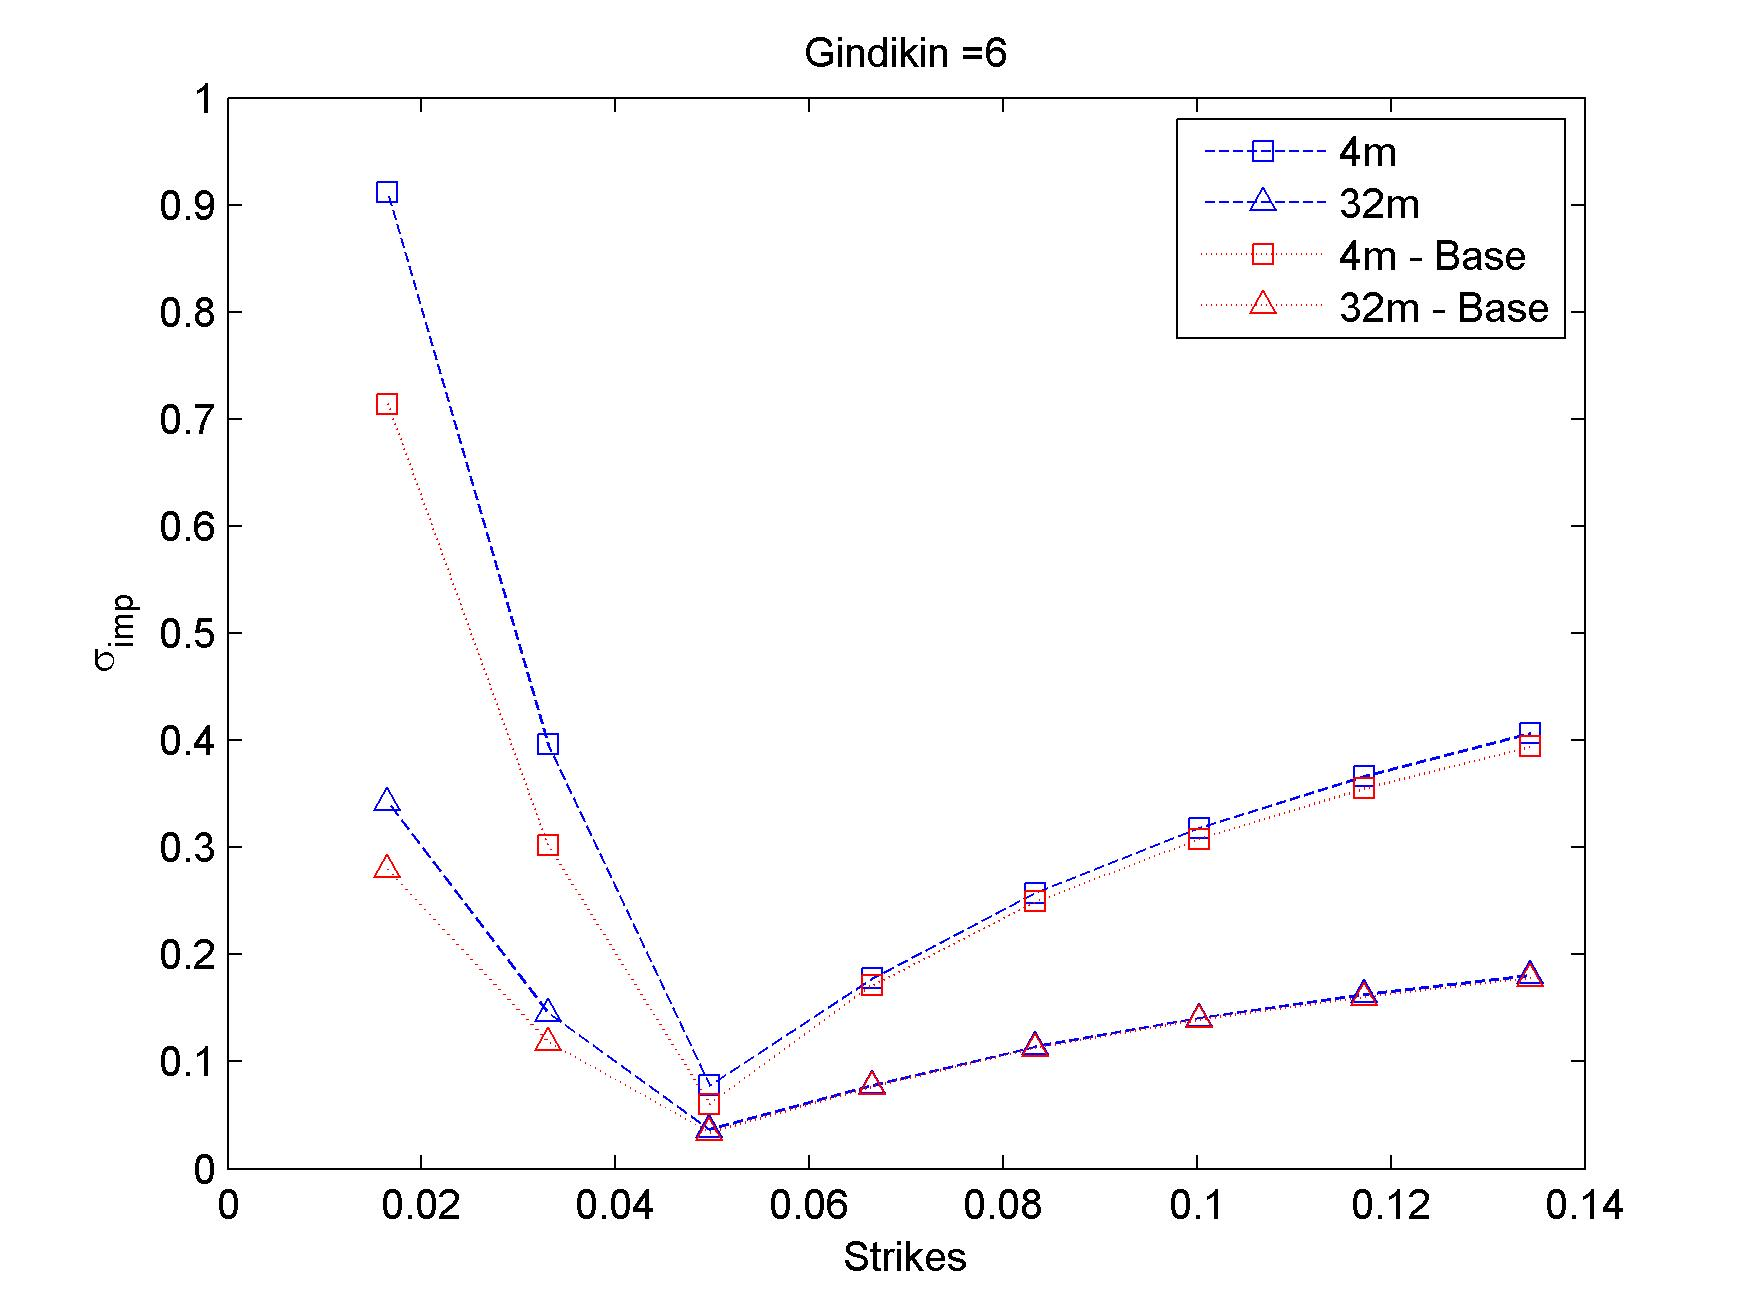
\includegraphics[scale=0.14]{figure1.jpg}
\caption{Doubling $\kappa$ with respect to the basic case causes an upward shift of the surface. The plot represents the two smiles (4 months and 32 months) for the basic ($\kappa =3$) and the modified case ($\kappa = 6$).}\label{fig:1}
\end{figure}

\begin{figure}[H]
  \centering
  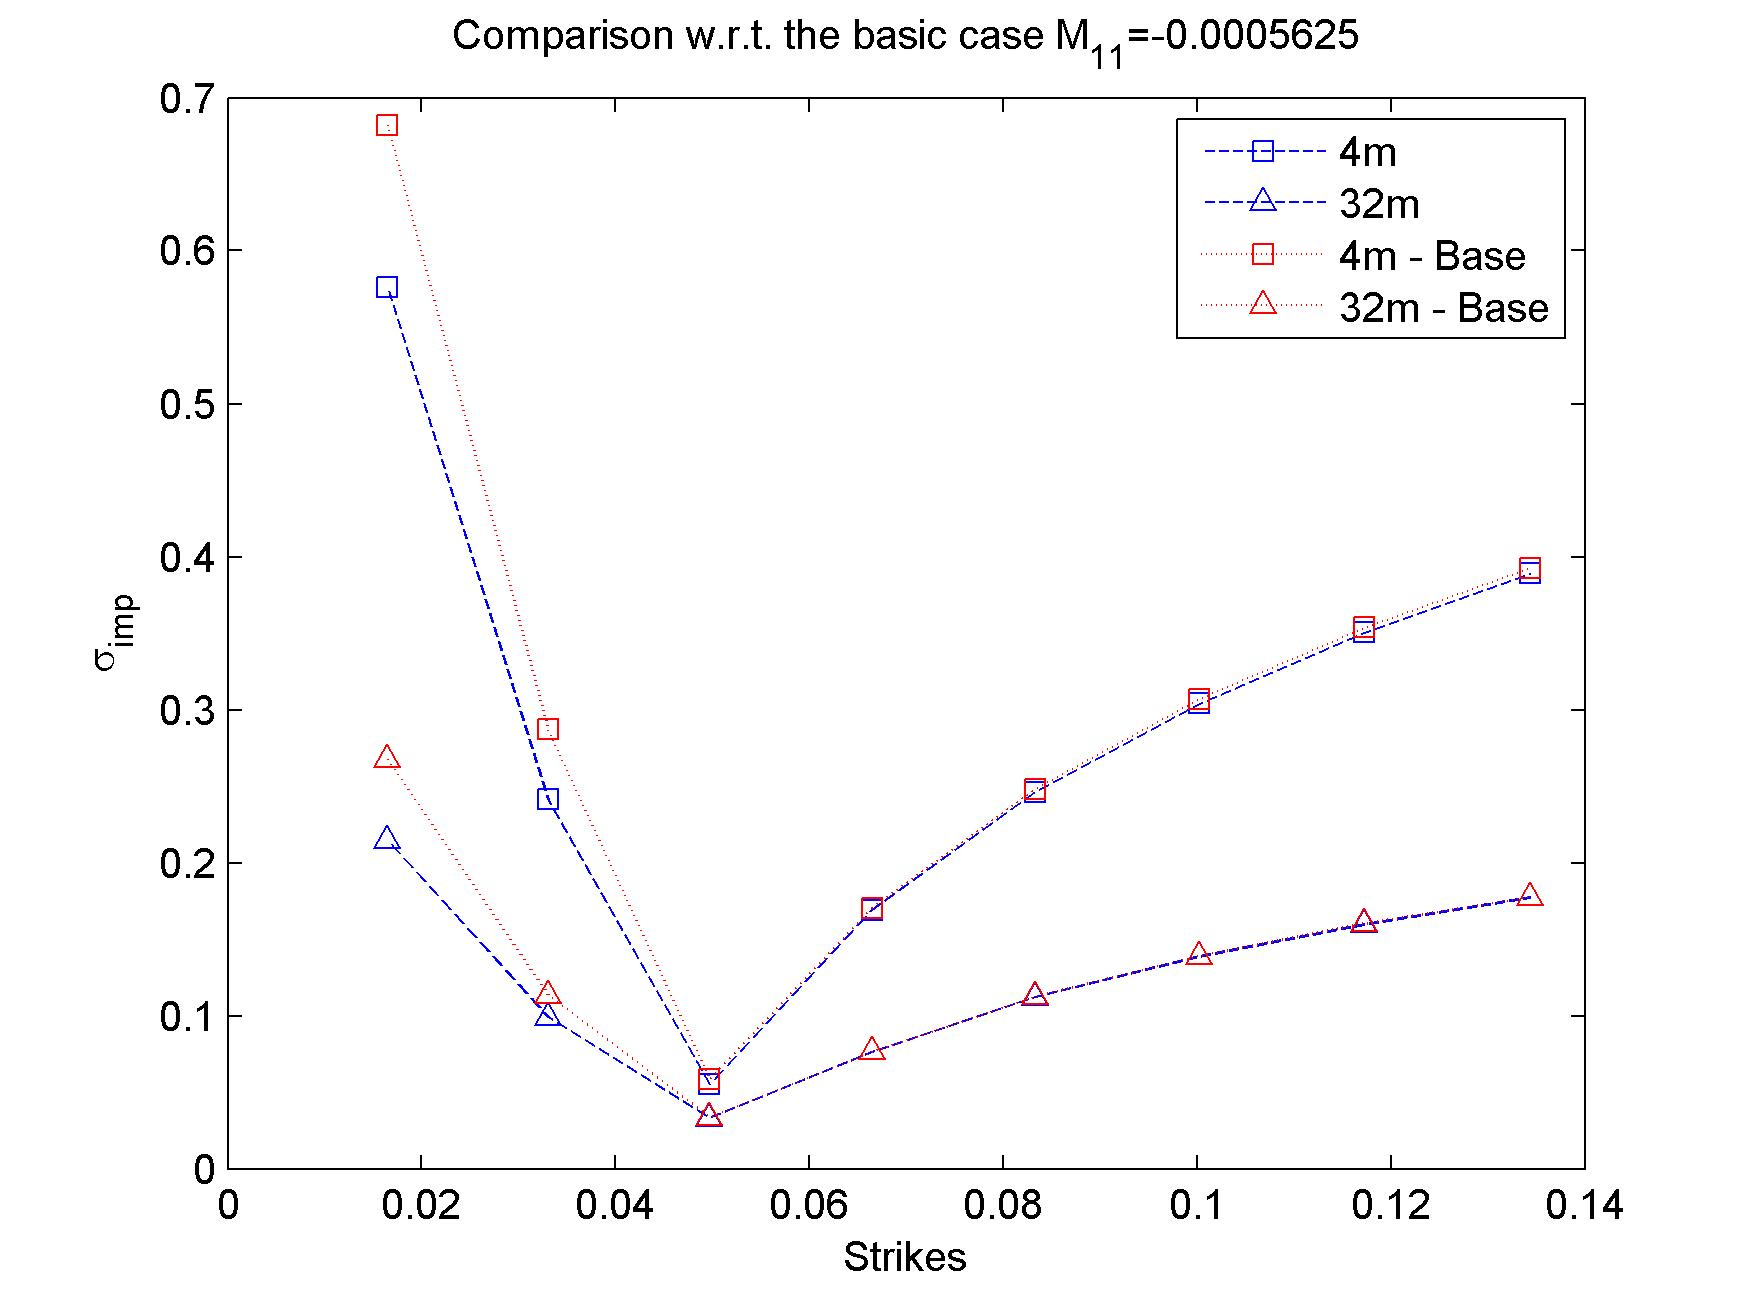
\includegraphics[scale=0.14]{figure2.jpg}
  \caption{Impact of $M_{11}$. $M_{11}$ is negative and the present image shows the effects on the two smiles (4 months and 32 months) we obtain when we multiply it by a constant $c=1.8$}
  \label{fig:2}
\end{figure}

\begin{figure}[H]
  \centering
  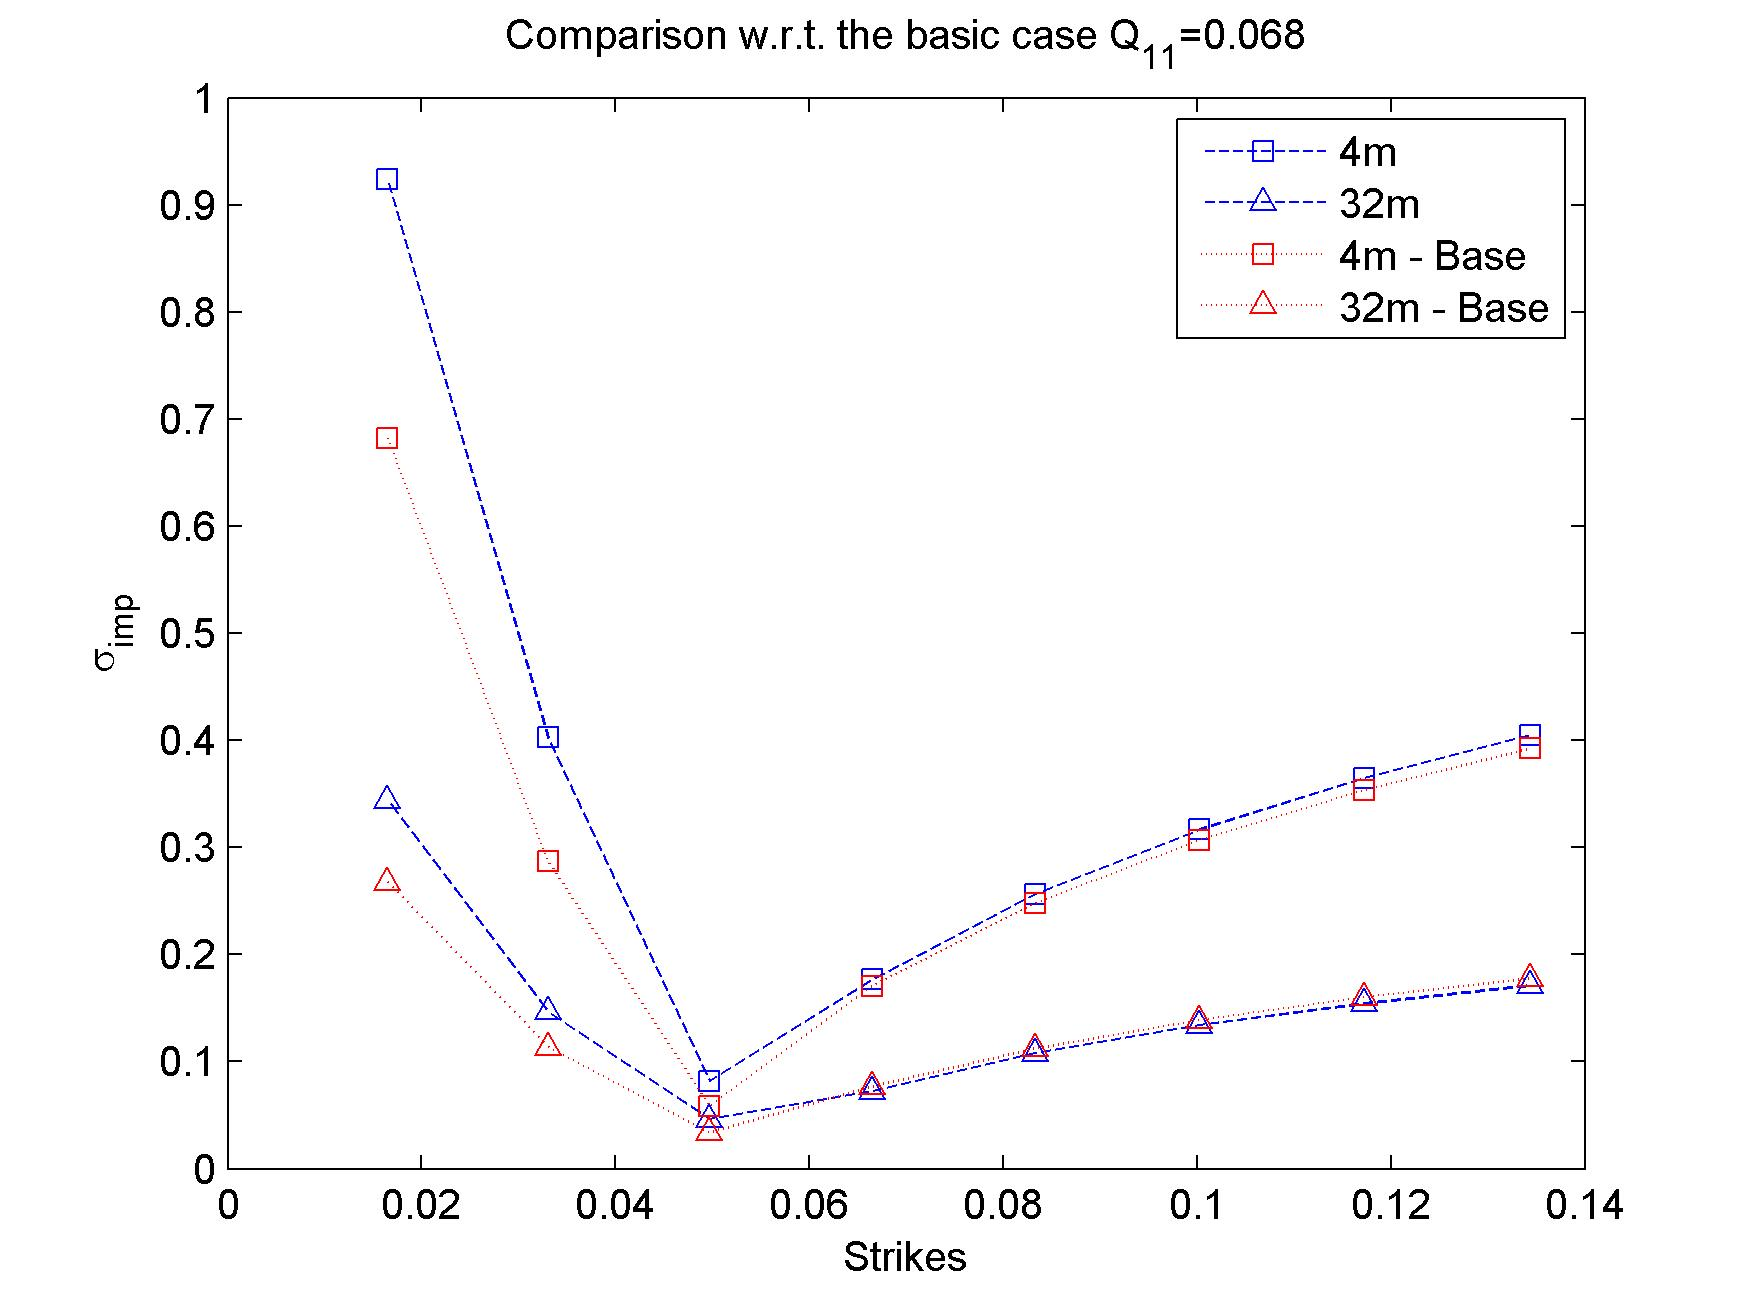
\includegraphics[scale=0.18]{figure3.jpg}
  \caption{Impact of $Q_{11}$. $Q_{11}$ is positive and the present image shows the effects on the two smiles (4 months and 32 months) we obtain when we multiply it by a constant $c=2$}
  \label{fig:3}
\end{figure}

\begin{figure}[H]
  \centering
  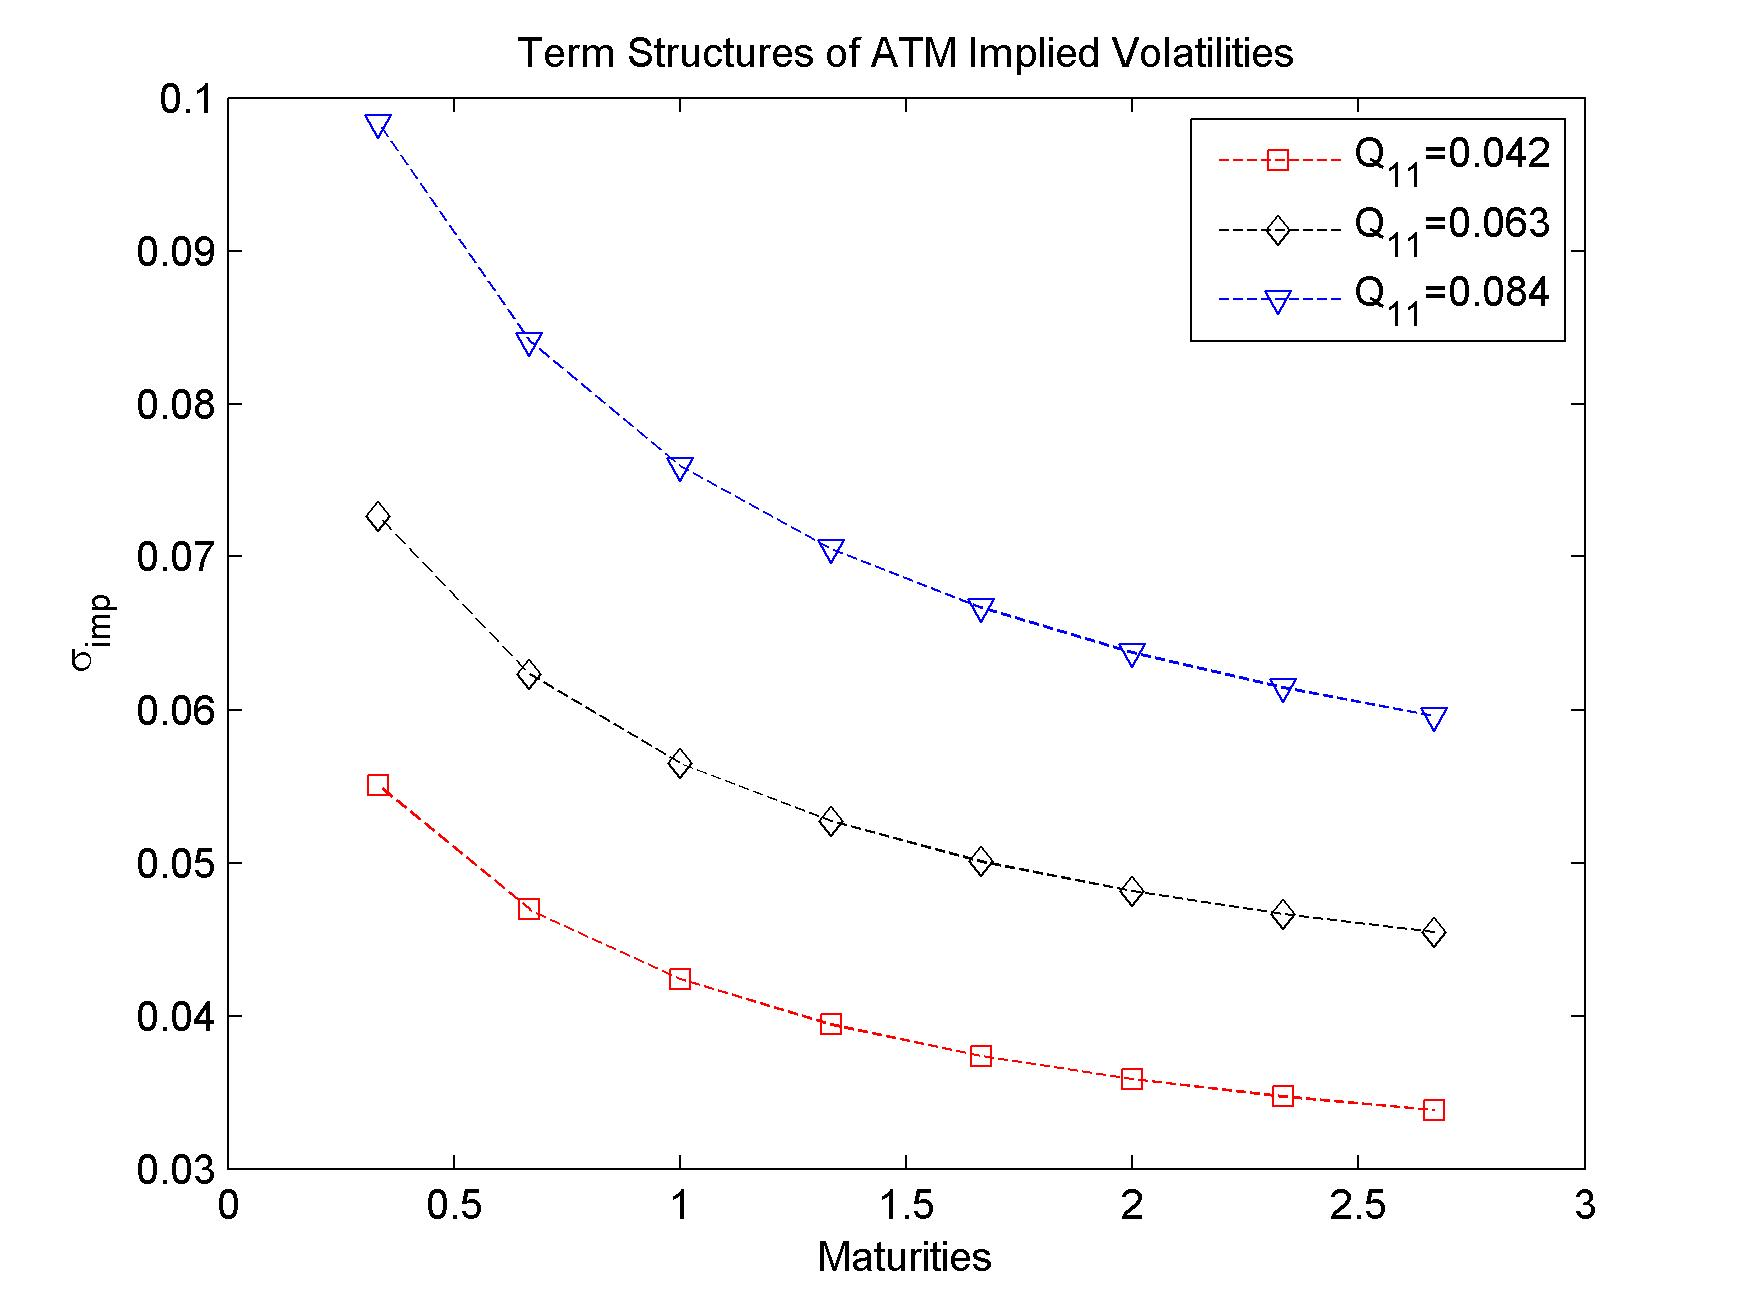
\includegraphics[scale=0.18]{figure4.jpg}
  \caption{Impact of $Q$ on the term structures of ATM implied volatilities. Here we consider $Q_{11}$ and multiply its value by a constant $c=1,1.5,2$ so as to get the values in the legend.}
  \label{fig:4}
\end{figure}

\begin{figure}[H]
  \centering
  \subfloat{\label{fig:fig21}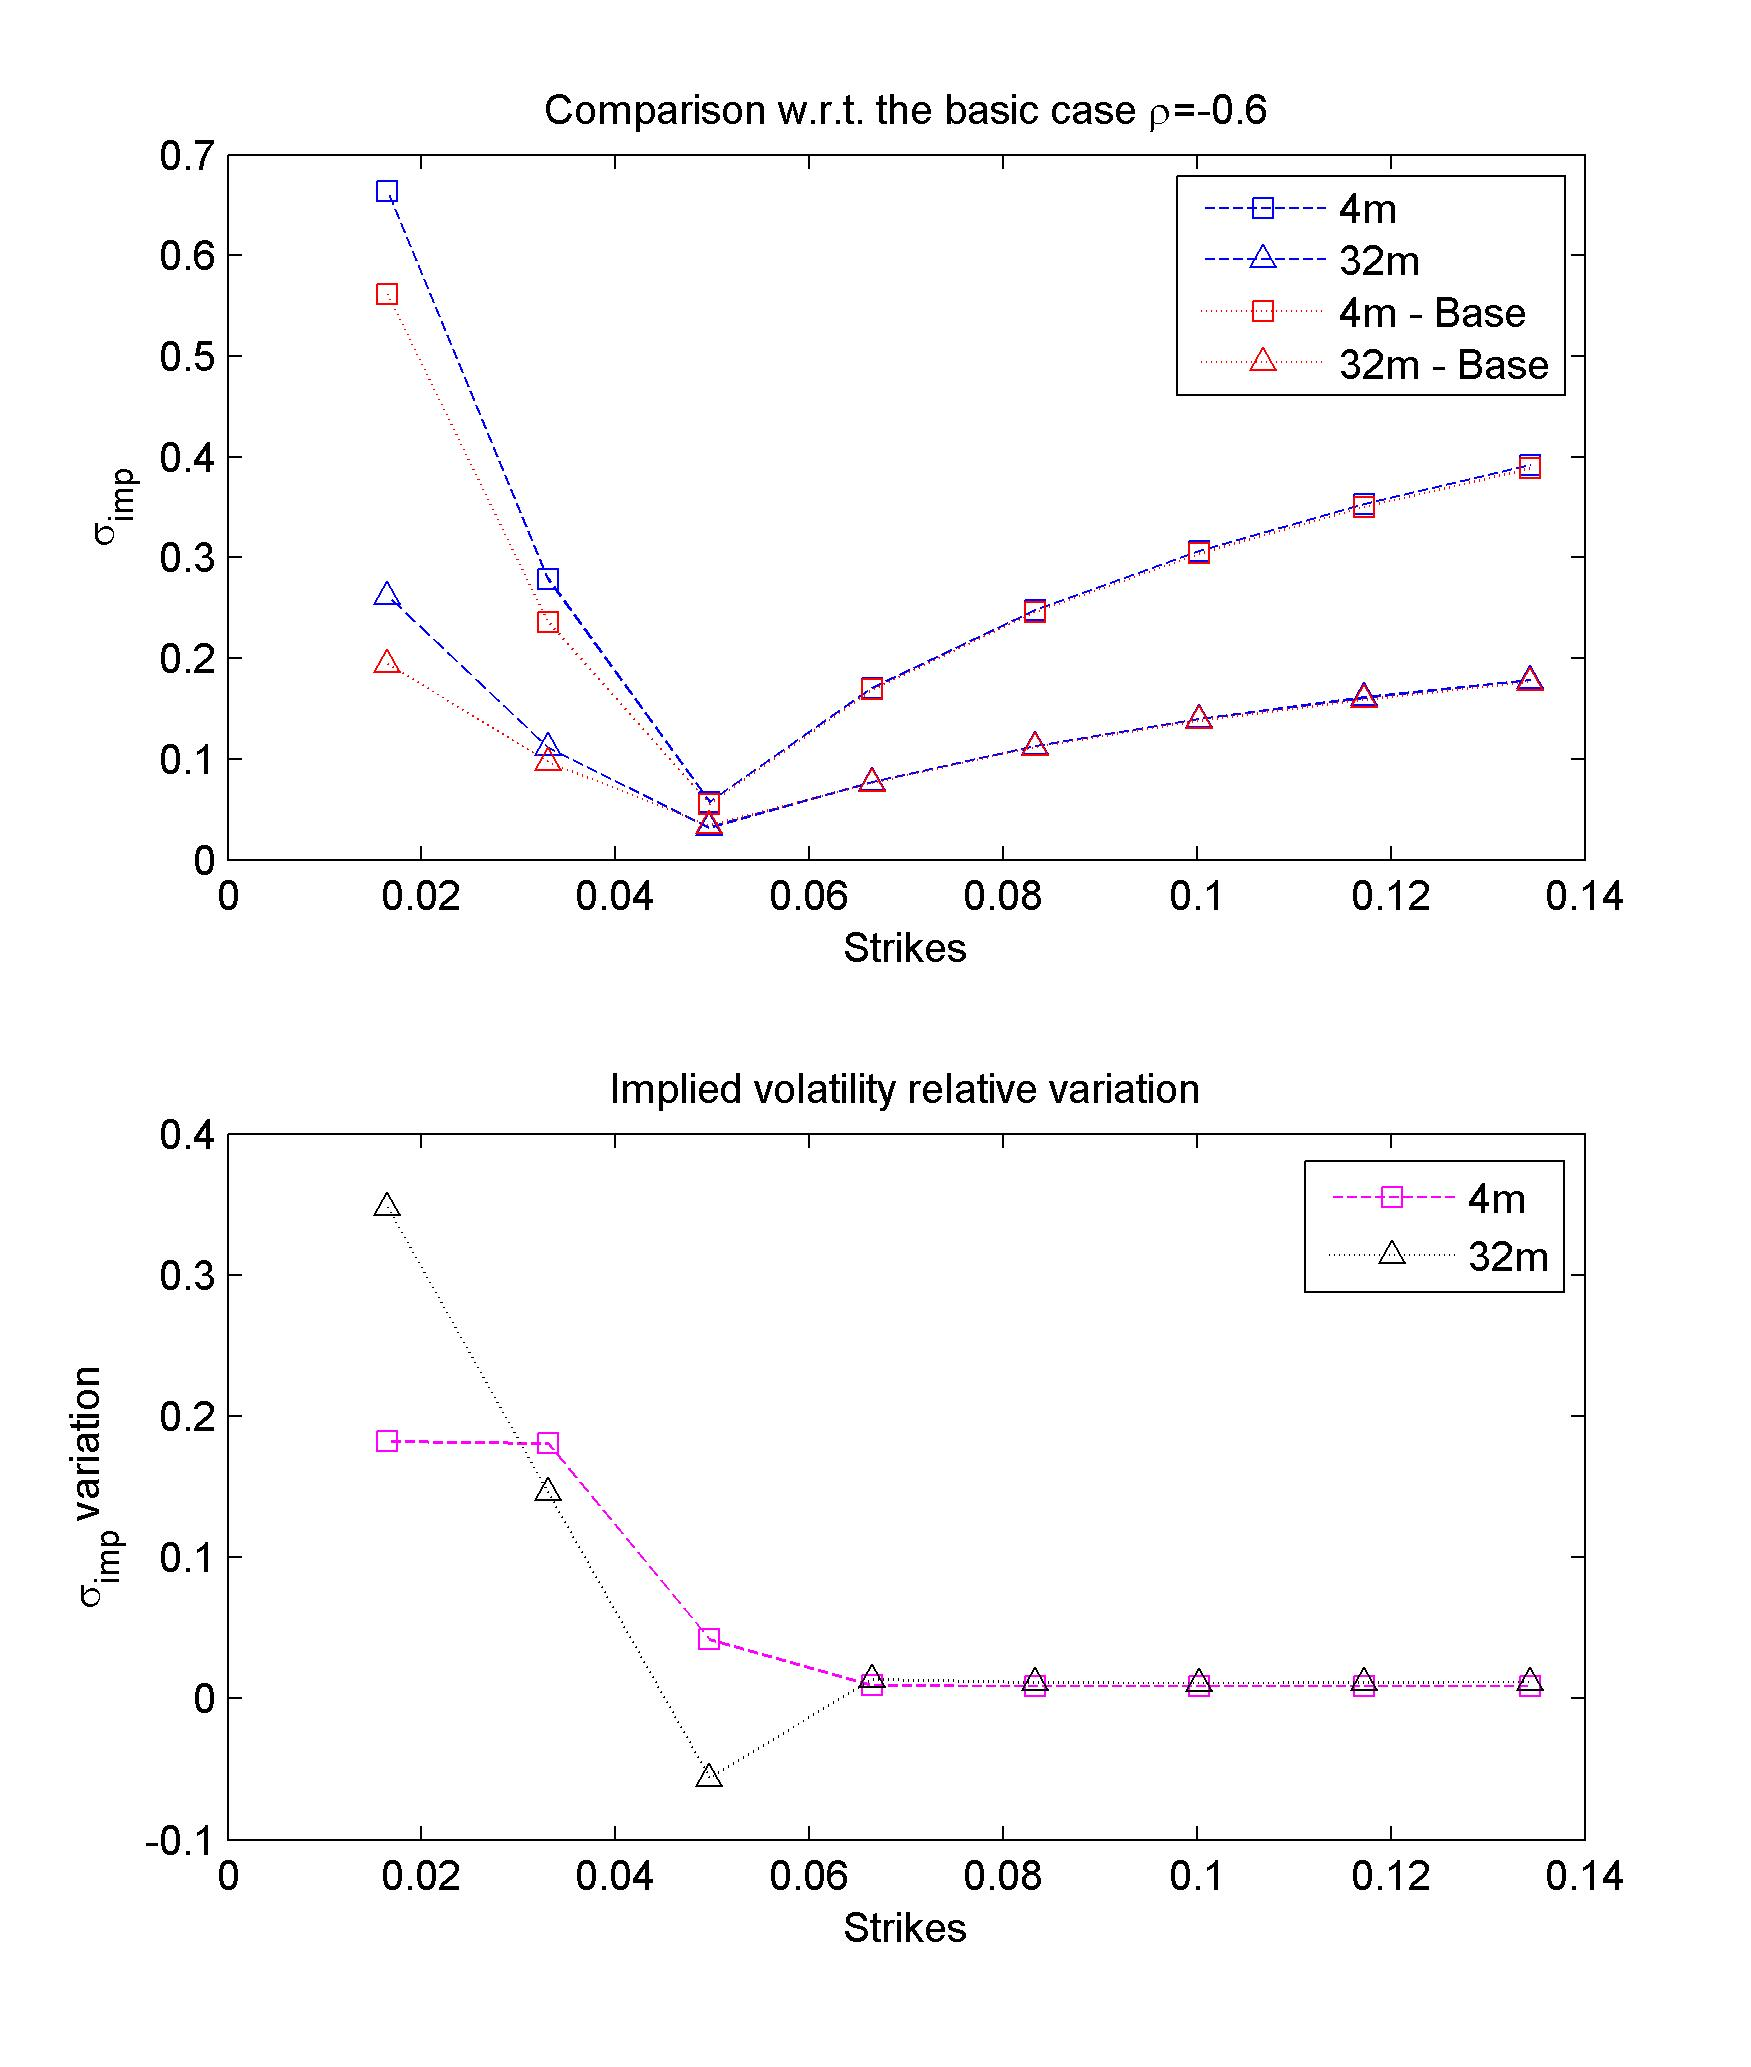
\includegraphics[width=0.5\textwidth]{figure5.jpg}}                
  \subfloat{\label{fig:fig22}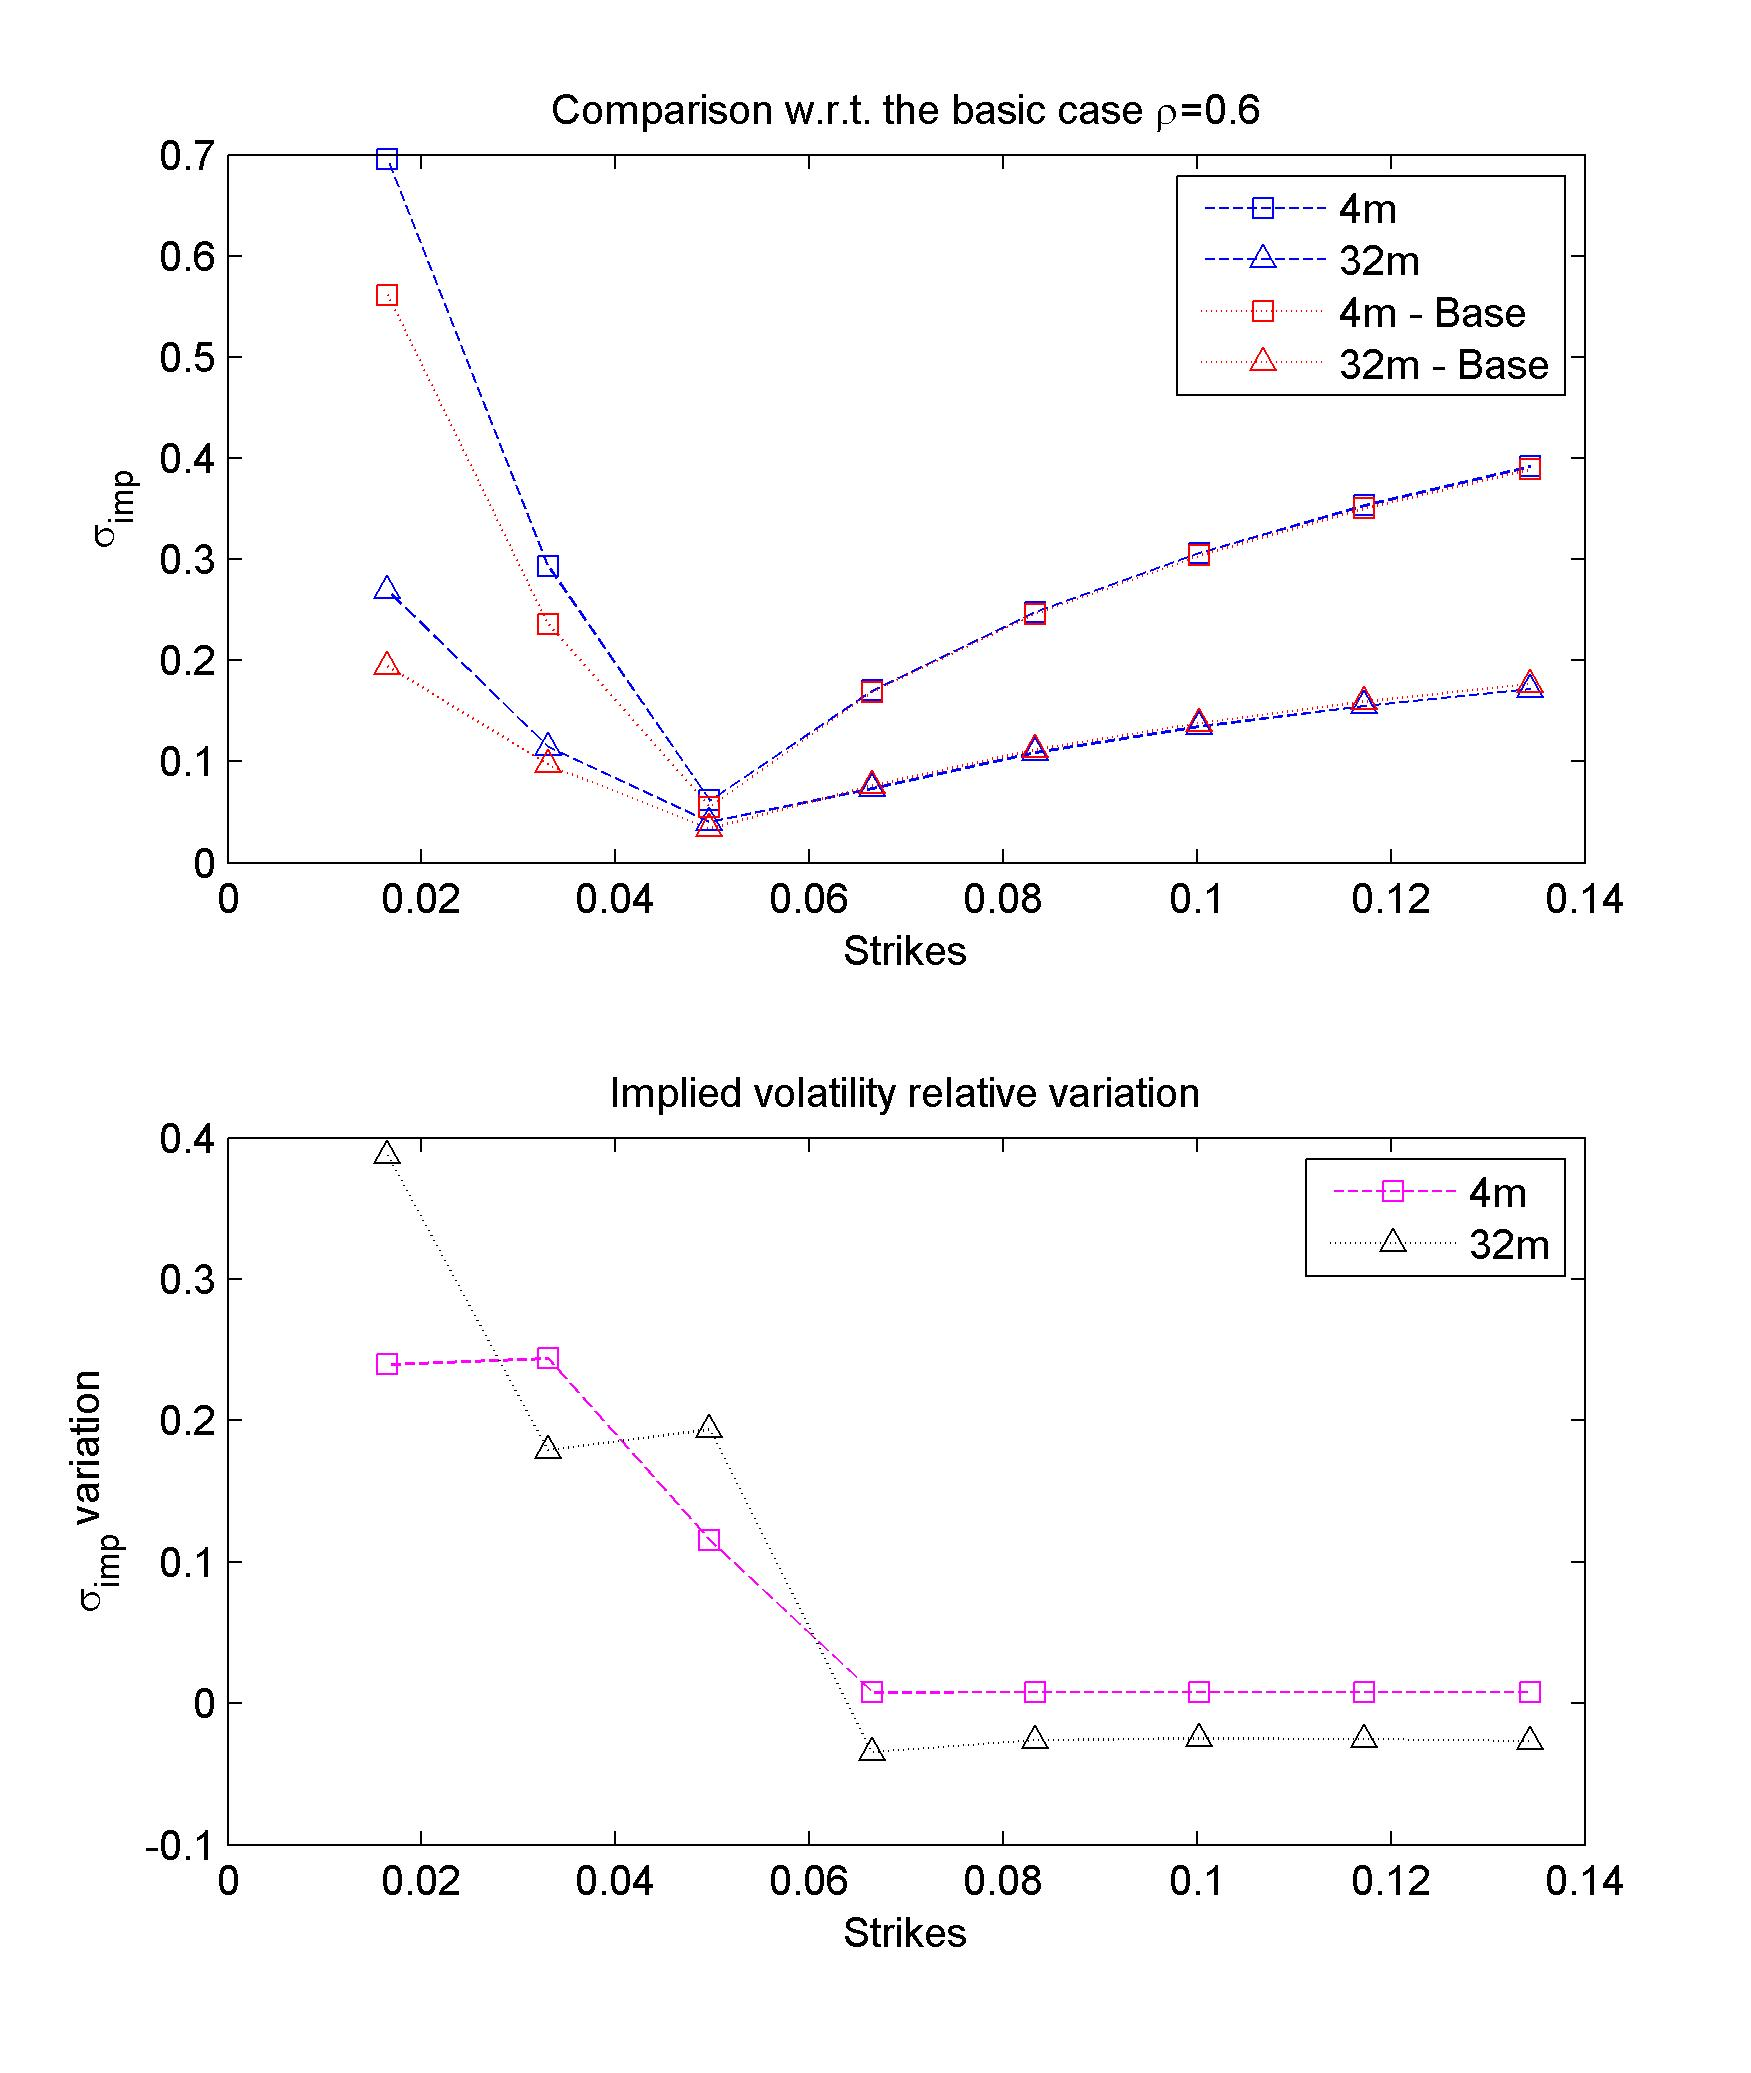
\includegraphics[width=0.5\textwidth]{figure6.jpg}}               
\caption{The images above highlight the flexibility of the Wishart Libor model. We are able to impose different patterns to the term structure of ATM implied volatility. On the top we have the smiles and on the bottom we observe the relative changes of the smiles, i.e. for every point of the smiles we calculate the quantity $\left(\sigma^{imp}_{final}-\sigma^{imp}_{initial}\right)/\sigma^{imp}_{initial}$. Notice in particular the situation on the left side, where we observe around 5\% (ATM) an increase of the short term smile and a decrease on the long term.}
  \label{fig:5}
\end{figure}

\begin{figure}[H]
\centering
  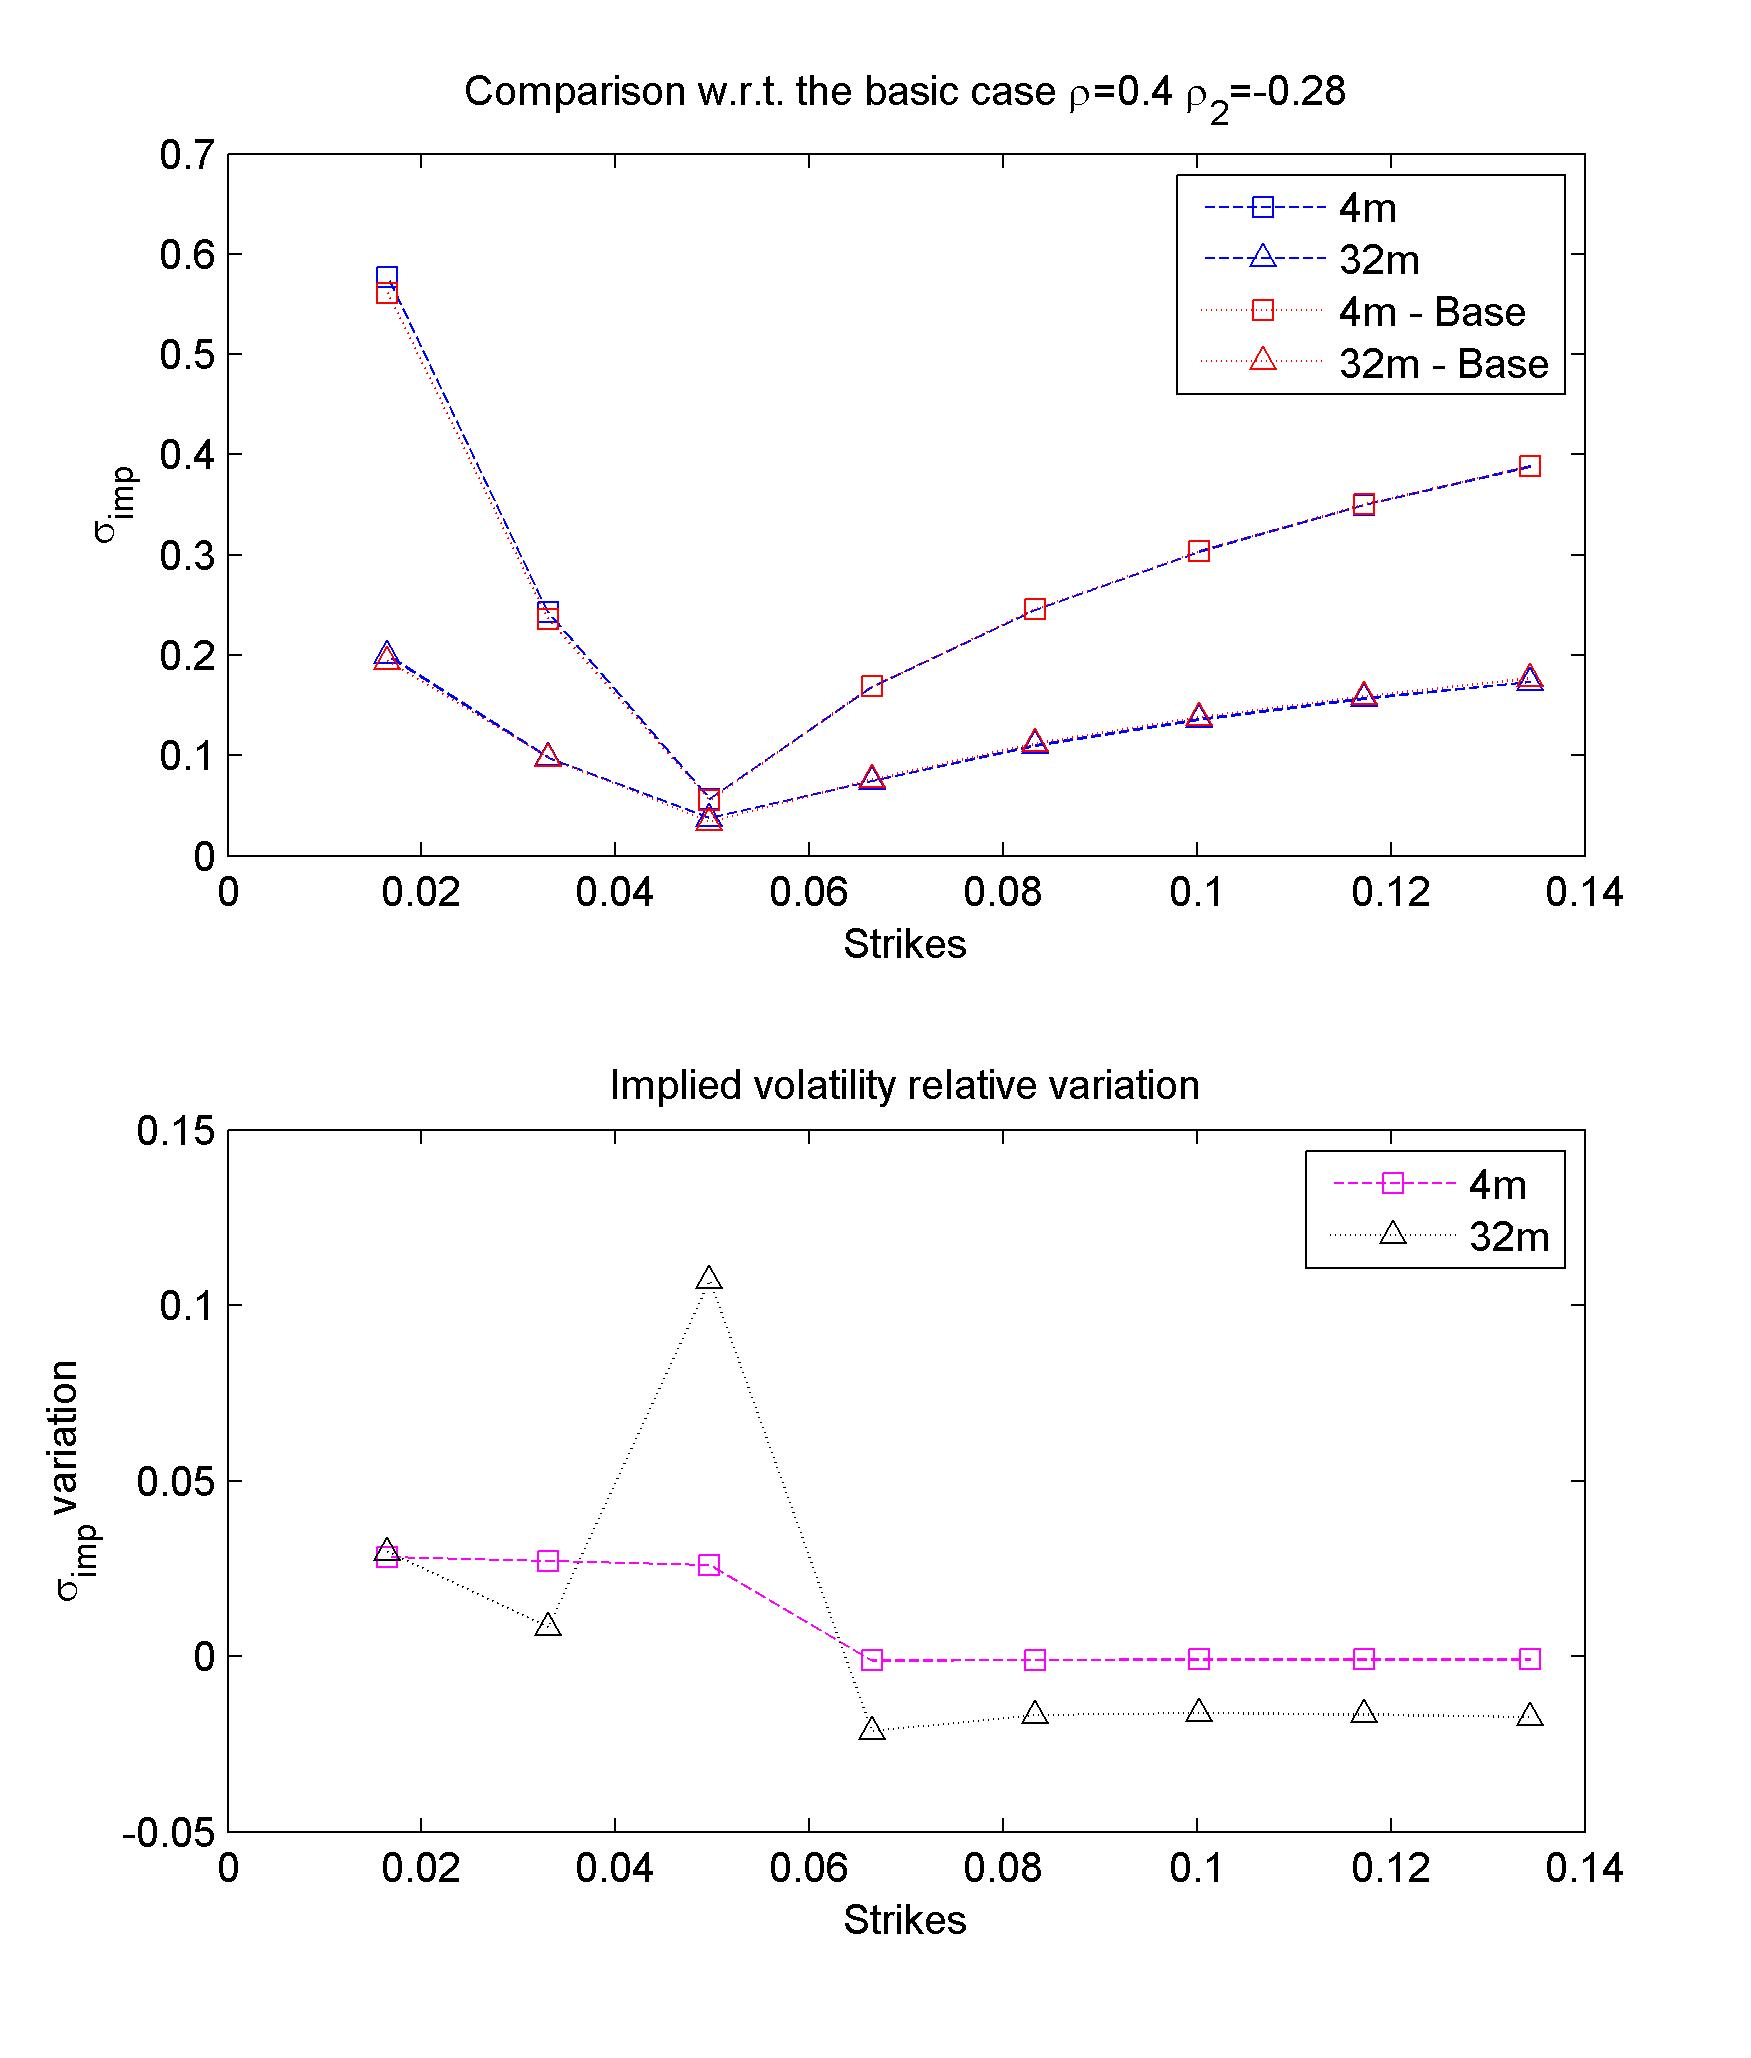
\includegraphics[scale=0.18]{figure9.jpg}
  \caption{Impact on the implied volatility surface when both $M$ and $Q$ are parametrized as symmetric matrices. Notice the level around 5\%, corresponding to ATM. This shows that if we parametrize both $M$ and $Q$ via $\rho,\rho_2$ we have a flexible setting which is controlled just by two parameters that allow us to perform different combinations. In particular $\rho$ and $\rho_2$ have opposite impacts in the present example ($\rho>0$ whereas $\rho_2<0$), meaning that we have a good degree of control.}
  \label{fig:9}
\end{figure}

\begin{figure}[H]
\centering
  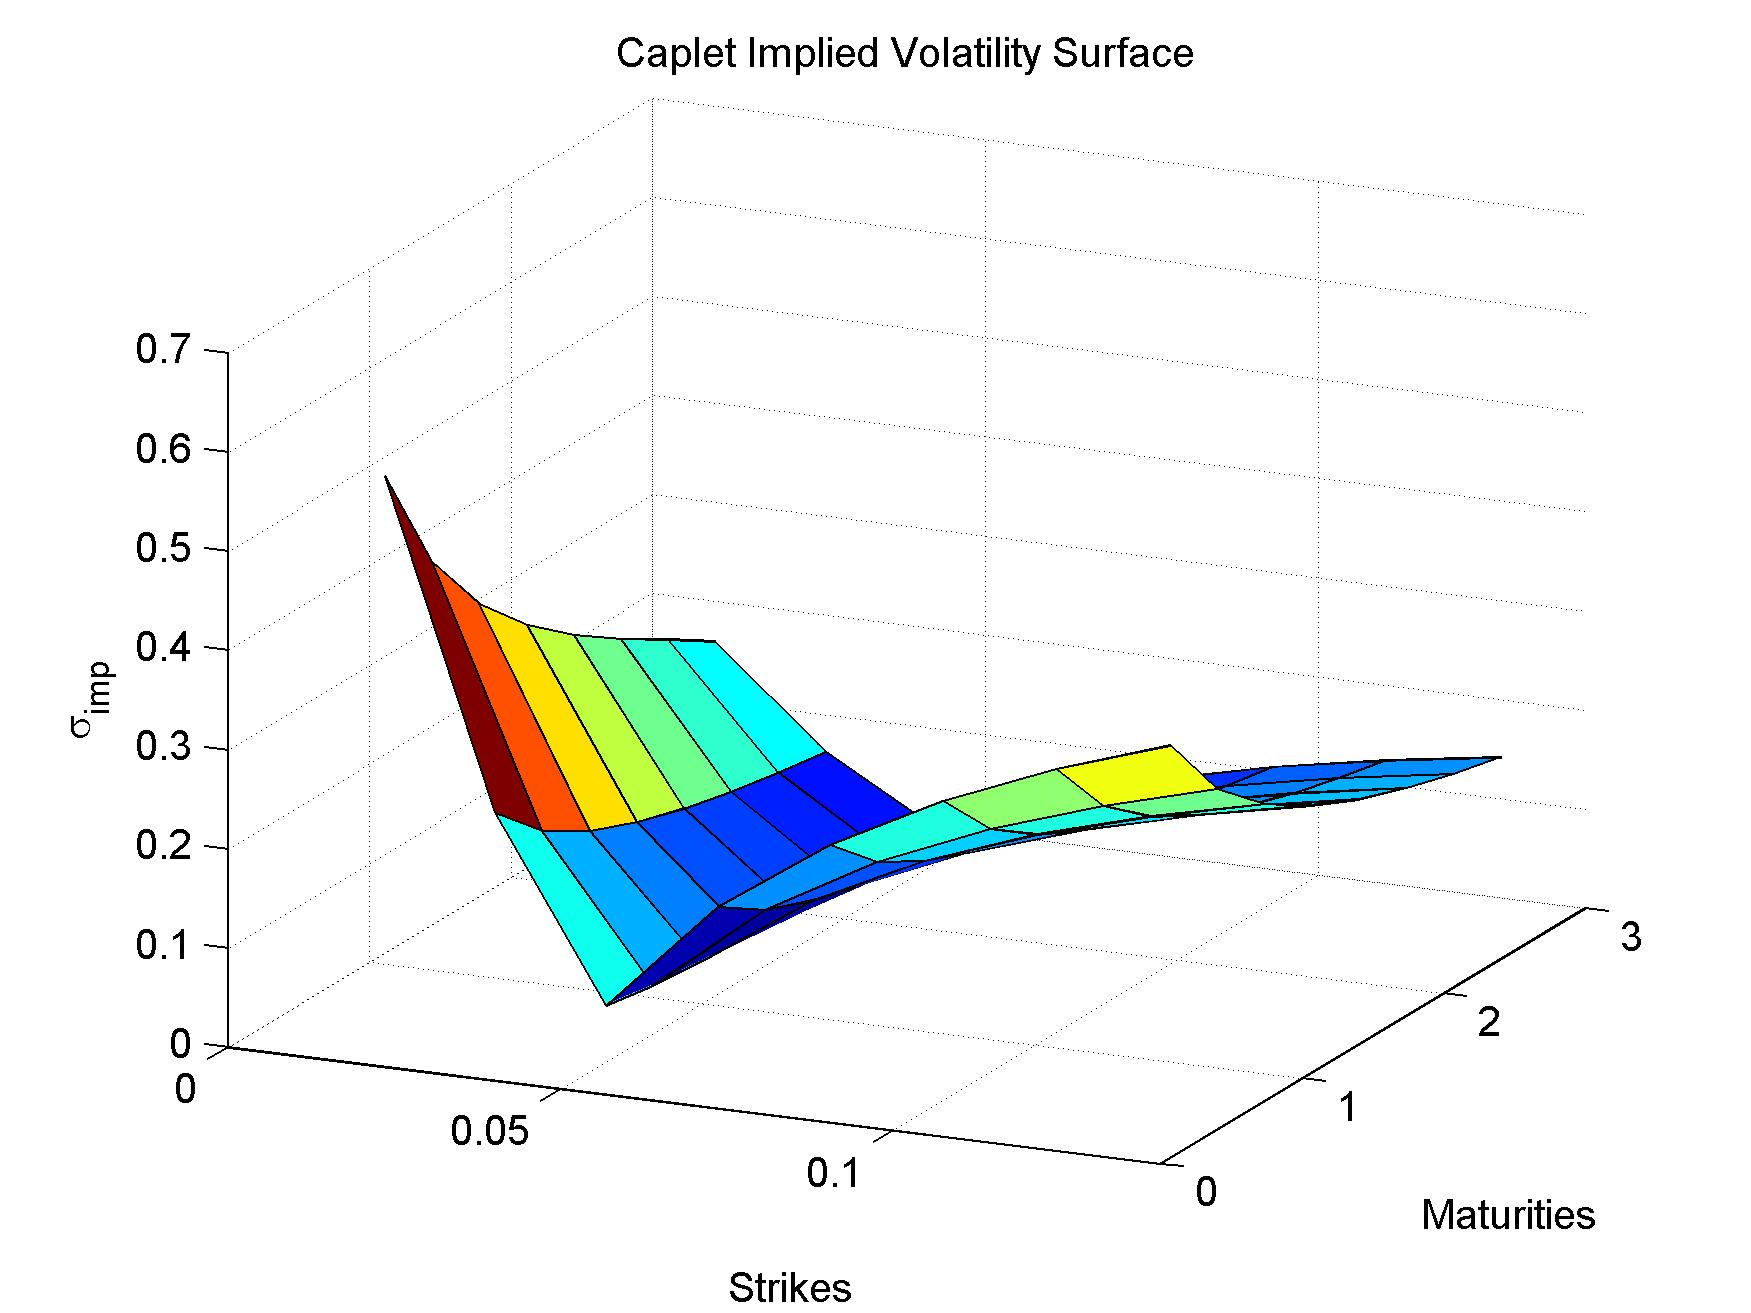
\includegraphics[scale=0.18]{figure7.jpg}
  \caption{Caplet Implied Volatility Surface generated by the Wishart Libor model}
  \label{fig:7}
\end{figure}

\begin{figure}[H]
\centering
  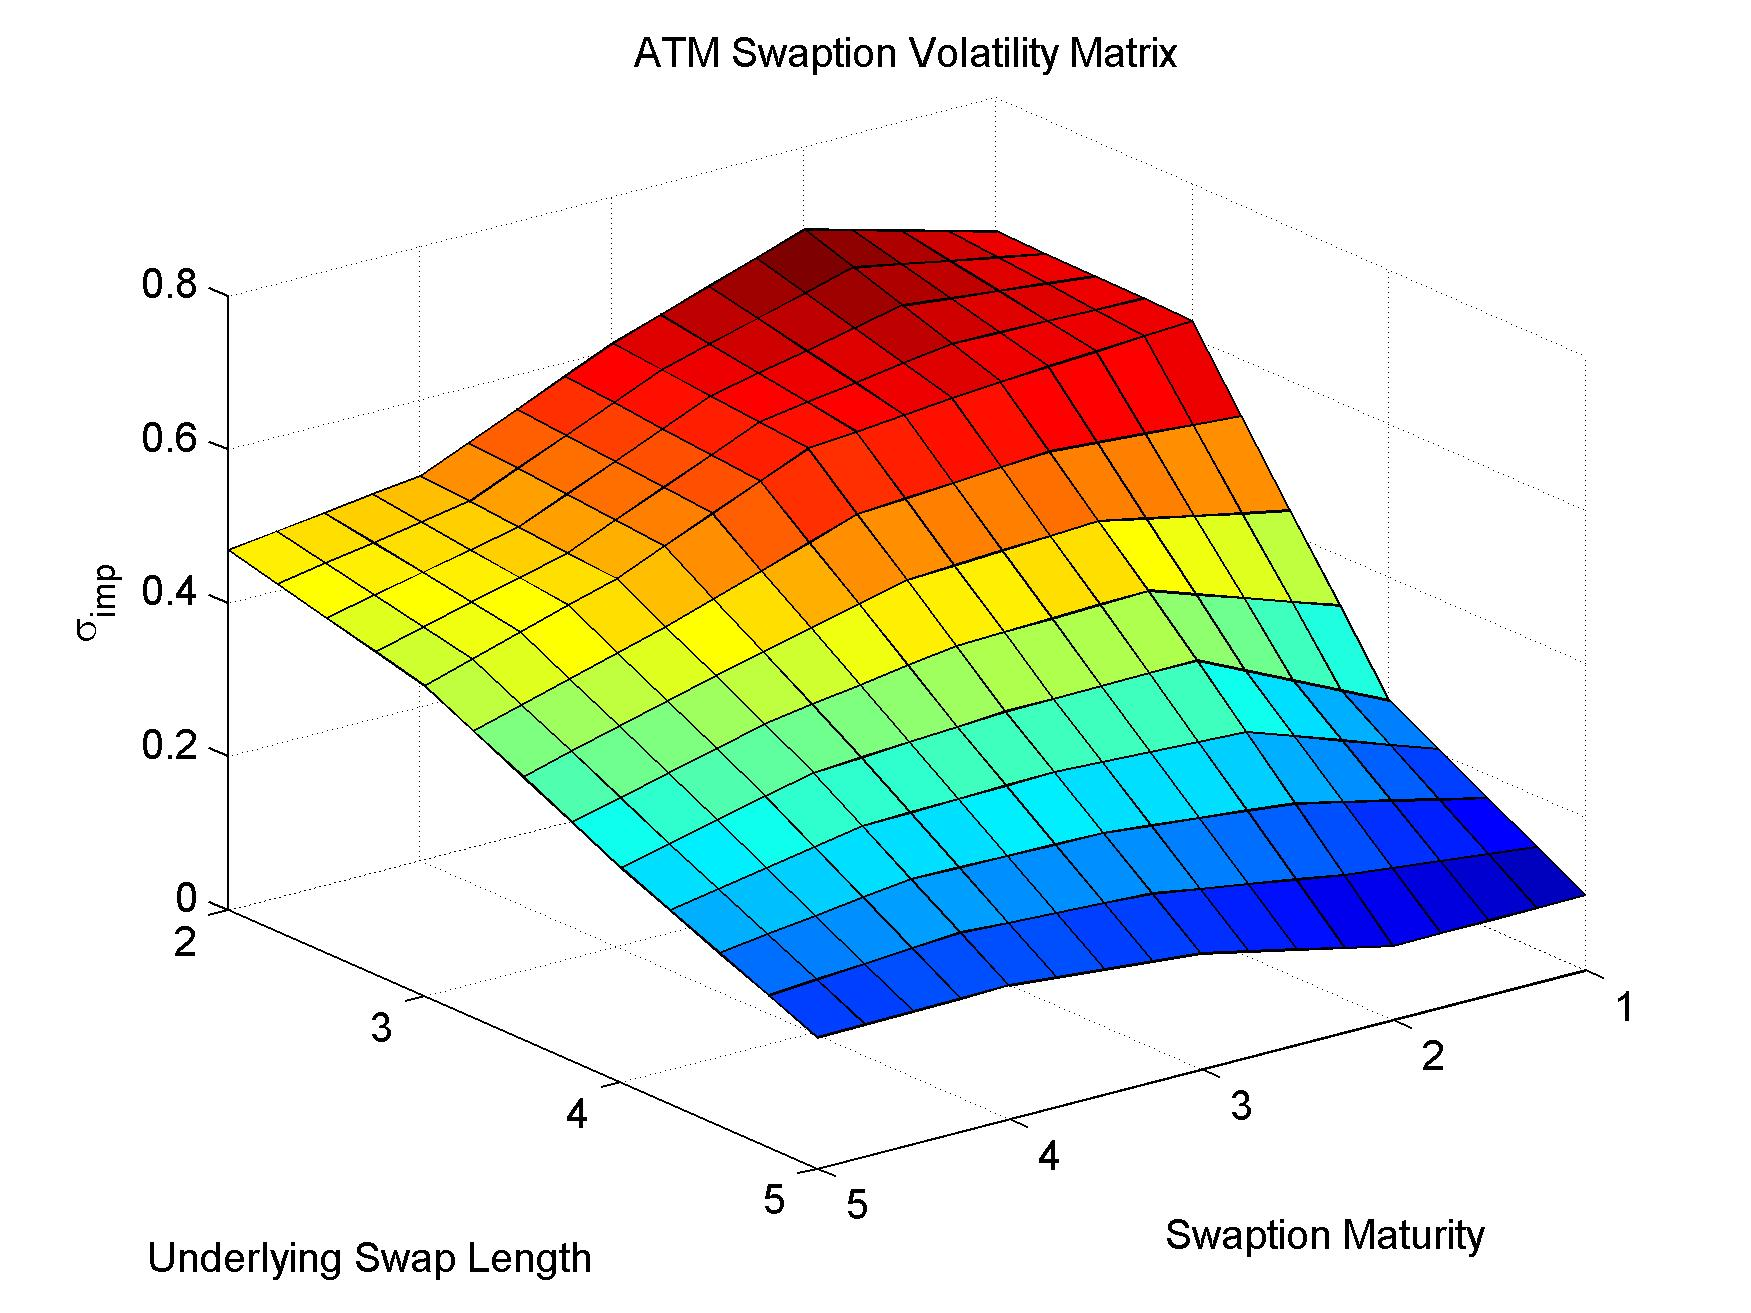
\includegraphics[scale=0.18]{figure8.jpg}
  \caption{ATM Swaption Implied Volatility Surface generated by the Wishart Libor model}
  \label{fig:8}
\end{figure}


\begin{figure}[H]
\centering
  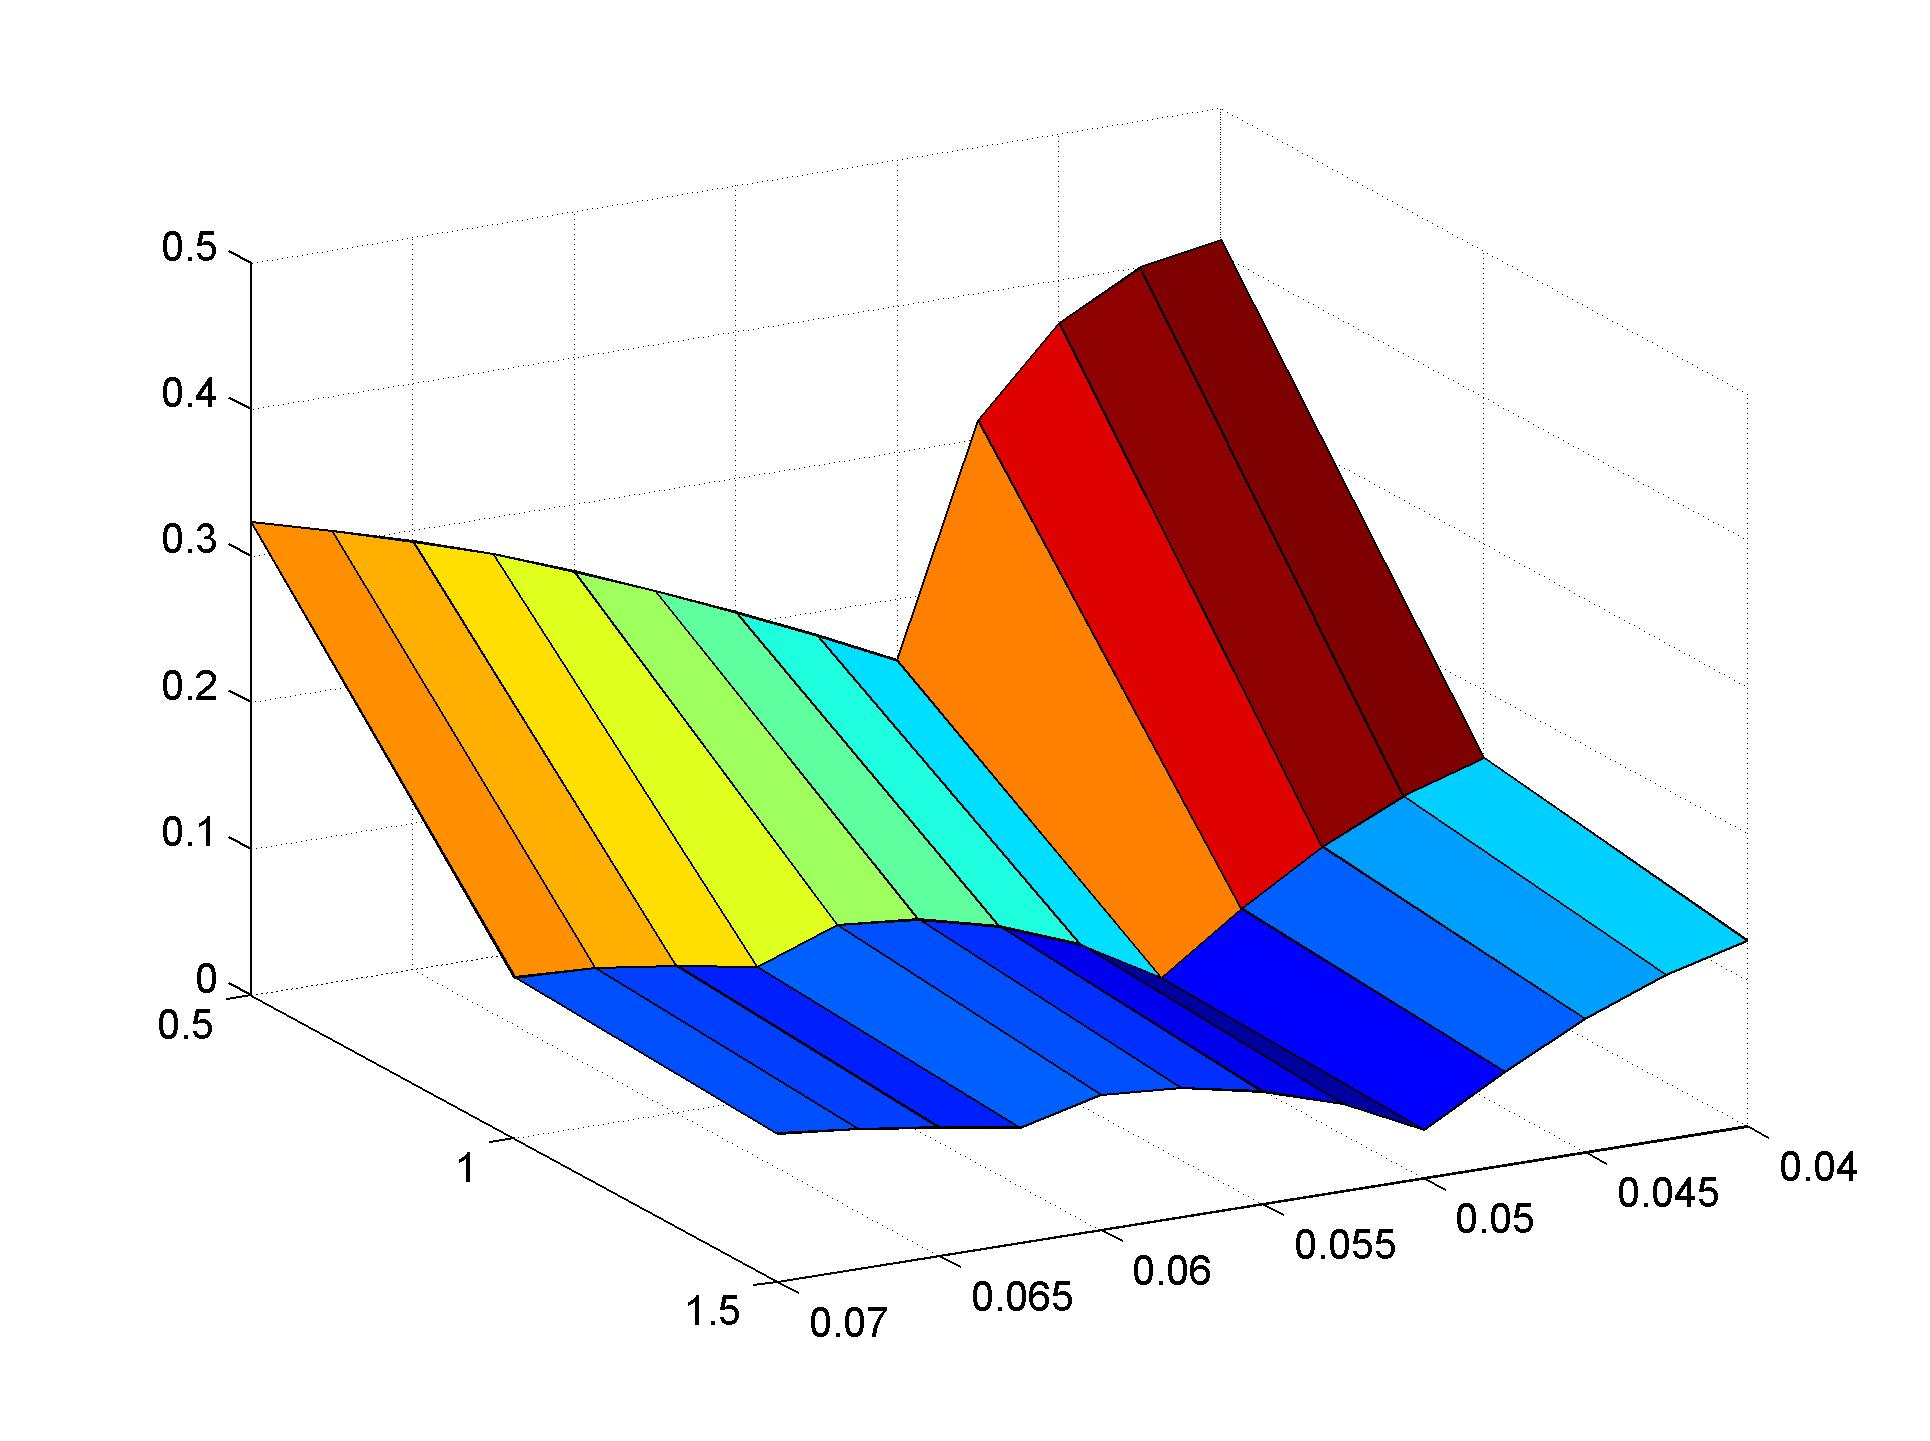
\includegraphics[scale=0.18]{JumpFig01.jpg}
  \caption{Caplet Implied Volatility Surface generated by the compound Poisson Libor model with Wishart distributed jumps}
  \label{fig:10}
\end{figure}


